%%%%%%%%%%%%%%%%%%%%%%%%%%%%%%%%%%%%%%%%%%%%%%%%%%%%%%%%%%%%

\chapter{Background and Related Work}\label{chap:background}
To generate a vector representation of named entities and terms in an annotated document, we use either a corpus of text with entity annotations or an co-occurrence graph extracted from it. Unlike traditional methods, where all tokens are treated as terms, entity embeddings take the type information into account.To provide a general background for all the methods used in this work the related work is organized as follows:\\
First, a brief overview of the text preprocessing steps for NLP tasks is given, in which methods used to extract information from text and generate a co-occurrence graph are explained. In Section~\ref{sec:nn} neural network based approaches for learning embeddings is explained. The co-occurrence graphs are explained in Section~\ref{sec:graph} along with the LOAD~\brackettext{\cite{DBLP:conf/sigir/SpitzG16}} model, which is specific co-occurrence graph used in this study.  Since word2vec and GloVe are the building blocks of other models they are described in Section~\ref{sec:wordembeddig}. In this section, we also explain how the edge weights of the co-occurrence graph can be used to generate a weighted adjacency matrix, which is comparable to a co-occurrence matrix in the GloVe model.  Finally, an overview of the some of the important graph embedding methods is given in Section~\ref{sec:graph}. These models are used on the co-occurrence graphs in Chapter~\ref{chap:entity} and~\ref{chap:faceted} to create the entity and faceted embeddings respectively. 

\section{Basics of Natural Language Processing}
The goal of NLP systems is to understand and derive meaning from human language. Textual data is a valuable source of information in NLP. Most of the World Wide Web is made of text, with websites like Twitter generating vast amounts every day. Analyzing this content is, however, not a simple task. For example, text might contain ambiguity, as in the sentence \emph{``I put my \textbf{wallet} in the  \textbf{car}.  \textbf{It} is green.''} In this sentence, it is not obvious if \emph{``it''} refers to the \emph{``car''} or the  \emph{``wallet''}. Moreover, humans often use homographs (words having the same spelling but different meanings), metaphors and sarcasm, which makes text analysis even more challenging. \\
As machine learning systems rely on features, the most important step is to derive features from the text. Multiple models have been proposed for feature extraction, while none of them achieve the goal of fully characterizing a text, some are more useful than others. However, all features require cleaning and preprocessing of the text. 

\subsection{Text cleaning }
Before any operation can be performed on text, each sentence has to be broken down to its atomic pieces. \emph{Tokenization} is the act of chopping sentences up into pieces, called \emph{tokens}.  For example, the sentence: \emph{Tokenization is widely used in Natural Language Processing}, can be tokenized as follows : \\

\mybox{Tokenization} \mybox{is} \mybox{widely} \mybox{used} \mybox{in} \mybox{natural language processing}.\\
\\
Splitting only into white spaces can also split what should be regarded as a single token. In a later section, we discuss \emph{named entity recognition} that tries to eliminate such problems.  \\
\noindent
Text data has many inconsistencies that can cause algorithms trouble. Some common initial preprocessing steps are to convert all of the letters to lowercase and to remove punctuation. 
This makes sure that \emph{``analytics"}, \emph{``AnALYticS"}, \emph{``Analytics!"}, and \emph{``\#analytics"} are all considered the same word. Removing punctuation should be applied with care as in some cases, such as in case of Twitter \emph{``\#analytics"} is a message about analytics and should not be confused with \emph{``@analytics"}, which is a message to the analytics account. For these reasons, the removal of punctuation should be tailored to the specific problem.\\
Additionally, words such as \emph{``are"} and \emph{``to"} are frequent in all documents but are only meaningful in a sentence. These are called \emph{stop-words}. Despite the high frequency, these words are unlikely to result in a meaningful feature for a machine learning system and are often removed. As with punctuation, removing stop words blindly may result in loss of valuable information. For example, \emph{``The Who"} is the name of a band, which by removing the stop-words, we remove both of these words, but it might have a significant meaning~\brackettext{\cite{SCHOL:edx/MIT15071}}. Hence, removing all stop-words is not always helpful, but it is generally a useful step. 

\subsection{Stemming and  lemmatization}
Another important preprocessing step is \emph{stemming} or \emph{lemmatization}. This step is motivated by the desire to represent words with different endings as the same word. In many cases, there is no need for a distinction between \emph{argue}, \emph{argued}, \emph{argues}, and \emph{arguing}. They could all be represented by a common stem: \emph{argu}. This is called stemming as it chops off the ends of words and often includes the removal of derivational affixes. Another approach is the use of lemmatization, which uses the vocabulary and morphological analysis of words, normally aiming to remove inflectional endings only and to return the base or dictionary form of a word, which is known as the lemma. lemmatization is a more complex task as it is necessary to have detailed dictionaries which the algorithm can look through to link the form back to its lemma. For instance:
Lemmatization of drank is drink~\brackettext{\cite{SCHOL:book/larson2010}}.
\subsection{Part-Of-Speech tagging (POStagging)}
\emph{POS tagging} is the process of marking up a word in a text corresponding to a particular part of speech. Parts of speech are also known as \emph{word classes} or \emph{lexical categories} (e.g., noun, verb, adjective,~\dots). POS tags are useful because of a large amount of information they give about a word and its neighbors and also about the syntactic context around the word. Parts of speech are useful features for finding named entities like people or organizations in text~\brackettext{\cite{SCHOL:book/jurafsky2016}}. \emph{POS taggers} are the software used to assign tags to tokens using a finite predefined tagset. For English, the most commonly used tagset is the \textbf{Penn Treebank POS tagset} \footcite{https://www.ling.upenn.edu/courses/Fall_2003/ling001/penn_treebank_pos.html}. 
\subsection{Named entity recognition and  entity linking}
\emph{Named entity recognition} (NER) or \emph{entity extraction} is an information extraction method that locates and classifies the named entities in text. Entities are classified into a set of pre-defined classes, such as the names of persons, organizations, locations, quantities and monetary values. In some case, temporal expressions are classified separately as well. Generally, anything that is not an entity per se is considered to be a term.~\brackettext{\cite{SCHOL:journal/LI/nadeau}}. More formally, if we consider all the words as terms and define $T$ as the set of all terms in the vocabulary, $N\subseteq T$ is the set of all entities that fall into a pre-defined category. Recognition of entities is difficult, partly because of ambiguity and mostly because of multiple surface forms. It is not always clear what is or is not an entity or what type it has. For example, the entity \emph{``Washington"} can be a name of a city, a person or even an organization. NER identifies the occurrence or mention of a named entity in the text, but it does not identify which specific entity it is. \emph{Named entity linking (NEL)}  or \emph{named entity disambiguation (NED)}  is the task of mapping the found entities to a repository of entities. For this purpose, \emph{knowledge bases} are used, which contain rich information about the entities and their mutual relationships. NEL maps the found entities to their corresponding pair in the knowledge base~\brackettext{\cite{DBLP:journals/tkde/ShenWH15}}. To generate the LOAD network, both of these methods were used to identify and disambiguate entities in the given corpus. These entities form the graph nodes in later steps. 

\section{Neural Networks  in Natural Language Processing }\label{sec:nn}
Before the advancements in deep learning and neural networks, most NLP techniques were based on machine-learning approaches with linear models such as support vector machines or logistic regression, trained on very high dimensional and sparse feature vectors. Recently, the field has changed to use non-linear neural-network models over dense inputs. The most important advantage of such methods is that they can often be trained with a single end-to-end model and do not require traditional task-specific feature engineering~\brackettext{\cite{DBLP:journals/jair/Goldberg16}}. Methods for different NLP tasks differ in architectures of neural networks and feature representations. Since the focus of this thesis is on word embeddings, we will focus on the explanation of a simple neural network and basic ideas needed to generate word embeddings in the following. 
\subsection{Neural networks}
Despite neural networks being the new trend in machine learning, they are rather old algorithms, which were motivated by the goal of having a machine that mimic the brain. The sudden resurgence of neural networks is due to the fact that they are computationally expensive algorithms and require a huge amounts of data, which was not available and processable in the 80s and 90s. \\
\begin{figure}
\centering 
\resizebox{0.55\textwidth}{0.3\textwidth}{      
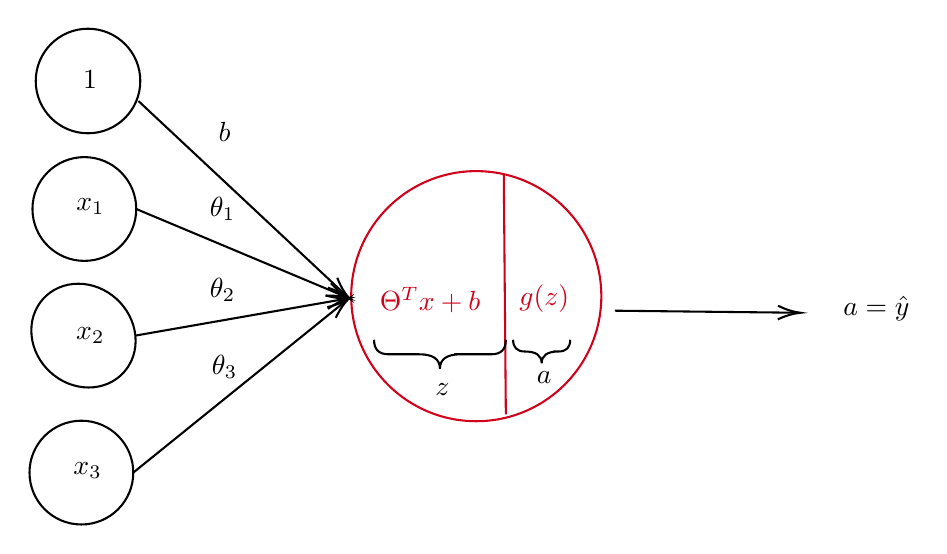
\begin{tikzpicture}[x=0.75pt,y=0.75pt,yscale=-1,xscale=1]
%uncomment if require: \path (0,300); %set diagram left start at 0, and has height of 300

%Shape: Circle [id:dp4894456216466021] 
\draw   (73.43,102) .. controls (73.43,88.19) and (84.63,77) .. (98.43,77) .. controls (112.24,77) and (123.43,88.19) .. (123.43,102) .. controls (123.43,115.81) and (112.24,127) .. (98.43,127) .. controls (84.63,127) and (73.43,115.81) .. (73.43,102) -- cycle ;
%Shape: Circle [id:dp5135503842228779] 
\draw   (73,163) .. controls (71.62,149.19) and (81.69,138) .. (95.5,138) .. controls (109.31,138) and (121.62,149.19) .. (123,163) .. controls (124.38,176.81) and (114.31,188) .. (100.5,188) .. controls (86.69,188) and (74.38,176.81) .. (73,163) -- cycle ;
%Shape: Circle [id:dp5054751399658592] 
\draw   (72,229) .. controls (72,215.19) and (83.19,204) .. (97,204) .. controls (110.81,204) and (122,215.19) .. (122,229) .. controls (122,242.81) and (110.81,254) .. (97,254) .. controls (83.19,254) and (72,242.81) .. (72,229) -- cycle ;
%Shape: Circle [id:dp7068247835752886] 
\draw  [color={rgb, 255:red, 208; green, 2; blue, 27 }  ,draw opacity=1 ] (227,144) .. controls (227,110.72) and (253.97,83.75) .. (287.25,83.75) .. controls (320.53,83.75) and (347.5,110.72) .. (347.5,144) .. controls (347.5,177.28) and (320.53,204.25) .. (287.25,204.25) .. controls (253.97,204.25) and (227,177.28) .. (227,144) -- cycle ;
%Straight Lines [id:da3951259360286594] 
\draw    (123.43,102) -- (224.16,144.23) ;
\draw [shift={(226,145)}, rotate = 202.75] [color={rgb, 255:red, 0; green, 0; blue, 0 }  ][line width=0.75]    (10.93,-3.29) .. controls (6.95,-1.4) and (3.31,-0.3) .. (0,0) .. controls (3.31,0.3) and (6.95,1.4) .. (10.93,3.29)   ;

%Straight Lines [id:da17712089576257095] 
\draw    (123,163) -- (224.03,145.34) ;
\draw [shift={(226,145)}, rotate = 530.0899999999999] [color={rgb, 255:red, 0; green, 0; blue, 0 }  ][line width=0.75]    (10.93,-3.29) .. controls (6.95,-1.4) and (3.31,-0.3) .. (0,0) .. controls (3.31,0.3) and (6.95,1.4) .. (10.93,3.29)   ;

%Straight Lines [id:da10379609280096158] 
\draw    (122,229) -- (224.44,146.26) ;
\draw [shift={(226,145)}, rotate = 501.07] [color={rgb, 255:red, 0; green, 0; blue, 0 }  ][line width=0.75]    (10.93,-3.29) .. controls (6.95,-1.4) and (3.31,-0.3) .. (0,0) .. controls (3.31,0.3) and (6.95,1.4) .. (10.93,3.29)   ;

%Straight Lines [id:da1555895906794451] 
\draw    (354,151) -- (441.5,151.98) ;
\draw [shift={(443.5,152)}, rotate = 180.64] [color={rgb, 255:red, 0; green, 0; blue, 0 }  ][line width=0.75]    (10.93,-3.29) .. controls (6.95,-1.4) and (3.31,-0.3) .. (0,0) .. controls (3.31,0.3) and (6.95,1.4) .. (10.93,3.29)   ;

%Shape: Circle [id:dp07492513539205437] 
\draw   (75,40.33) .. controls (75,26.42) and (86.28,15.14) .. (100.19,15.14) .. controls (114.1,15.14) and (125.38,26.42) .. (125.38,40.33) .. controls (125.38,54.24) and (114.1,65.52) .. (100.19,65.52) .. controls (86.28,65.52) and (75,54.24) .. (75,40.33) -- cycle ;
%Straight Lines [id:da37710728737628485] 
\draw    (124.5,50) -- (224.54,143.63) ;
\draw [shift={(226,145)}, rotate = 223.11] [color={rgb, 255:red, 0; green, 0; blue, 0 }  ][line width=0.75]    (10.93,-3.29) .. controls (6.95,-1.4) and (3.31,-0.3) .. (0,0) .. controls (3.31,0.3) and (6.95,1.4) .. (10.93,3.29)   ;

%Straight Lines [id:da9942335357246543] 
\draw [color={rgb, 255:red, 208; green, 2; blue, 27 }  ,draw opacity=1 ]   (300.5,85) -- (301.5,201) ;


%Shape: Brace [id:dp48208896309529936] 
\draw   (238,165) .. controls (238,169.67) and (240.33,172) .. (245,172) -- (259.75,172) .. controls (266.42,172) and (269.75,174.33) .. (269.75,179) .. controls (269.75,174.33) and (273.08,172) .. (279.75,172)(276.75,172) -- (294.5,172) .. controls (299.17,172) and (301.5,169.67) .. (301.5,165) ;
%Shape: Brace [id:dp308784031815875] 
\draw   (305,165) .. controls (305,168.77) and (306.89,170.66) .. (310.66,170.66) -- (310.66,170.66) .. controls (316.05,170.66) and (318.75,172.55) .. (318.75,176.32) .. controls (318.75,172.55) and (321.45,170.66) .. (326.84,170.66)(324.41,170.66) -- (326.84,170.66) .. controls (330.61,170.66) and (332.5,168.77) .. (332.5,165) ;

% Text Node
\draw (101.3,163) node   {$x_{2}$};
% Text Node
\draw (101.37,100.96) node   {$x_{1}$};
% Text Node
\draw (100,228) node   {$x_{3}$};
% Text Node
\draw (101.21,39.84) node   {$1$};
% Text Node
\draw (166,65) node   {$b$};
% Text Node
\draw (165,102) node   {$\theta _{1}$};
% Text Node
\draw (165,141) node   {$\theta _{2}$};
% Text Node
\draw (166,178) node   {$\theta _{3}$};
% Text Node
\draw (480,150) node   {$a=\hat{y}$};
% Text Node
\draw (320,145) node [color={rgb, 255:red, 208; green, 2; blue, 27 }  ,opacity=1 ]  {$g( z)$};
% Text Node
\draw (265,146) node [color={rgb, 255:red, 208; green, 2; blue, 27 }  ,opacity=1 ]  {$\Theta ^{T} x+b$};
% Text Node
\draw (271,189) node   {$z$};
% Text Node
\draw (320,183) node   {$a$};


\end{tikzpicture}


}
\caption{Single layer neural network. The input $x$ is multiplied by the weights $w$ to be passed to the neuron and generate the output $\hat { y }$~\brackettext{\cite{SCHOL:coursera/AndrewNg/DL}}.}
\label{fig:preceptron}
\end{figure}
A single artificial neuron is shown in Figure~\ref{fig:preceptron}. The computational unit illustrated in red takes in the different features $x$ and multiplies each input with a given weight $w$. The weights indicate the importance of each feature for the computation. The neuron then performs a non-linear transformation to the input and generates the output ($\hat { y } $). $b$ is called the \emph{bias unit} which always has an input value of $1$. $g(x)$ is called the \emph{activation
function} and represents the non-linear transformation that is applied on the input data. Essentially, each neuron consists of two steps of computation. First, $z$ is computed by the multiplication of weights and inputs. Second, an activation function of choice is applied to $z$ to produce the final output. The output or activation ($a$) of the last unit is the predicted output. A neural network is a group of multiple neurons connected together, as shown in Figure~\ref{fig:nn}. In a
neural network, the first layer is called the input layer and the last layer is called the output layer. Any layer in between is considered as a hidden layer. Typically, the values of the input and the output layer are given in the training set. Activation of each computational unit is the output of that unit after applying a certain function on the inputs, we denote activation of the unit (neuron) $i$ in layer $j$ by $a_{i}^{[j]}$. The $\theta^{(j)}_{nl}$ is the weight controlling the function mapping from layer $j$ to layer $j+1$ between unit $n$ in layer $j$ and $l$ in $j+1$. Learning this weight matrix is the final goal of any deep learning system. The weights indicate how different features of inputs should be combined and how much should each of them influence the final output. The values of intermediate activations can be interpreted as latent features discovered during training. Features are combined with new weights to either generate an intermediate or a final
result~\brackettext{\cite{SCHOL:online/AndrewNg/CS229,SCHOL:book/haykin2009}}. \\
\begin{figure}
\centering 
\resizebox{0.65\textwidth}{0.4\textwidth}{      
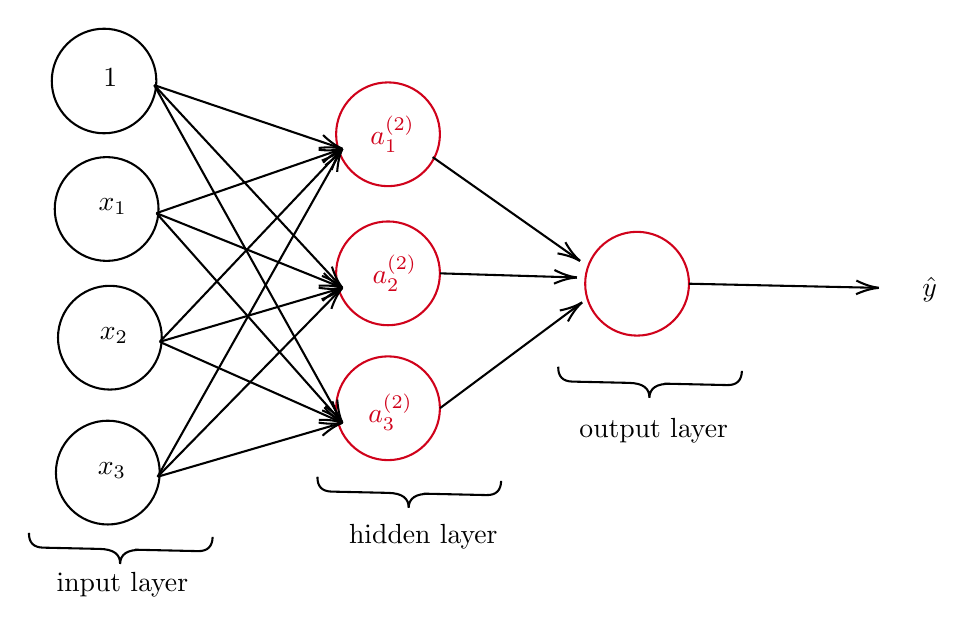
\begin{tikzpicture}[x=0.75pt,y=0.75pt,yscale=-1,xscale=1]
%uncomment if require: \path (0,300); %set diagram left start at 0, and has height of 300

\draw  [color={rgb, 255:red, 208; green, 2; blue, 27 }  ,draw opacity=1 ]  (241, 71) circle [x radius= 25, y radius= 25]  ;
\draw  [color={rgb, 255:red, 208; green, 2; blue, 27 }  ,draw opacity=1 ]  (241, 138) circle [x radius= 25, y radius= 25]  ;
\draw  [color={rgb, 255:red, 208; green, 2; blue, 27 }  ,draw opacity=1 ]  (241, 203) circle [x radius= 25, y radius= 25]  ;
\draw    (262.5,82) -- (333.5,132) ;
\draw [shift={(333.5,132)}, rotate = 215.15] [color={rgb, 255:red, 0; green, 0; blue, 0 }  ]   (0,0) .. controls (3.31,-0.3) and (6.95,-1.4) .. (10.93,-3.29)(0,0) .. controls (3.31,0.3) and (6.95,1.4) .. (10.93,3.29)   ;

\draw    (266,138) -- (332,140) ;
\draw [shift={(332,140)}, rotate = 181.74] [color={rgb, 255:red, 0; green, 0; blue, 0 }  ]   (0,0) .. controls (3.31,-0.3) and (6.95,-1.4) .. (10.93,-3.29)(0,0) .. controls (3.31,0.3) and (6.95,1.4) .. (10.93,3.29)   ;

\draw    (266,203) -- (334.5,152) ;
\draw [shift={(334.5,152)}, rotate = 503.33] [color={rgb, 255:red, 0; green, 0; blue, 0 }  ]   (0,0) .. controls (3.31,-0.3) and (6.95,-1.4) .. (10.93,-3.29)(0,0) .. controls (3.31,0.3) and (6.95,1.4) .. (10.93,3.29)   ;

\draw  [color={rgb, 255:red, 208; green, 2; blue, 27 }  ,draw opacity=1 ]  (361, 143) circle [x radius= 25, y radius= 25]  ;
\draw    (386,143) -- (477.5,145) ;
\draw [shift={(477.5,145)}, rotate = 181.25] [color={rgb, 255:red, 0; green, 0; blue, 0 }  ]   (0,0) .. controls (3.31,-0.3) and (6.95,-1.4) .. (10.93,-3.29)(0,0) .. controls (3.31,0.3) and (6.95,1.4) .. (10.93,3.29)   ;

\draw    (105.43, 107) circle [x radius= 25, y radius= 25]  ;
\draw    (107, 169) circle [x radius= 25, y radius= 25]  ;
\draw    (106, 234) circle [x radius= 25, y radius= 25]  ;
\draw    (104.19, 45.33) circle [x radius= 25.19, y radius= 25.19]  ;
\draw    (128.38,47.33) -- (219,78) ;
\draw [shift={(219,78)}, rotate = 198.7] [color={rgb, 255:red, 0; green, 0; blue, 0 }  ]   (0,0) .. controls (3.31,-0.3) and (6.95,-1.4) .. (10.93,-3.29)(0,0) .. controls (3.31,0.3) and (6.95,1.4) .. (10.93,3.29)   ;

\draw    (128.38,47.33) -- (219,145) ;
\draw [shift={(219,145)}, rotate = 227.14] [color={rgb, 255:red, 0; green, 0; blue, 0 }  ]   (0,0) .. controls (3.31,-0.3) and (6.95,-1.4) .. (10.93,-3.29)(0,0) .. controls (3.31,0.3) and (6.95,1.4) .. (10.93,3.29)   ;

\draw    (128.38,47.33) -- (219,210) ;
\draw [shift={(219,210)}, rotate = 240.88] [color={rgb, 255:red, 0; green, 0; blue, 0 }  ]   (0,0) .. controls (3.31,-0.3) and (6.95,-1.4) .. (10.93,-3.29)(0,0) .. controls (3.31,0.3) and (6.95,1.4) .. (10.93,3.29)   ;

\draw    (129.43,109) -- (219,210) ;
\draw [shift={(219,210)}, rotate = 228.43] [color={rgb, 255:red, 0; green, 0; blue, 0 }  ]   (0,0) .. controls (3.31,-0.3) and (6.95,-1.4) .. (10.93,-3.29)(0,0) .. controls (3.31,0.3) and (6.95,1.4) .. (10.93,3.29)   ;

\draw    (129.43,109) -- (219,145) ;
\draw [shift={(219,145)}, rotate = 201.9] [color={rgb, 255:red, 0; green, 0; blue, 0 }  ]   (0,0) .. controls (3.31,-0.3) and (6.95,-1.4) .. (10.93,-3.29)(0,0) .. controls (3.31,0.3) and (6.95,1.4) .. (10.93,3.29)   ;

\draw    (129.43,109) -- (219,78) ;
\draw [shift={(219,78)}, rotate = 520.9100000000001] [color={rgb, 255:red, 0; green, 0; blue, 0 }  ]   (0,0) .. controls (3.31,-0.3) and (6.95,-1.4) .. (10.93,-3.29)(0,0) .. controls (3.31,0.3) and (6.95,1.4) .. (10.93,3.29)   ;

\draw    (131,171) -- (219,78) ;
\draw [shift={(219,78)}, rotate = 493.42] [color={rgb, 255:red, 0; green, 0; blue, 0 }  ]   (0,0) .. controls (3.31,-0.3) and (6.95,-1.4) .. (10.93,-3.29)(0,0) .. controls (3.31,0.3) and (6.95,1.4) .. (10.93,3.29)   ;

\draw    (131,171) -- (219,145) ;
\draw [shift={(219,145)}, rotate = 523.54] [color={rgb, 255:red, 0; green, 0; blue, 0 }  ]   (0,0) .. controls (3.31,-0.3) and (6.95,-1.4) .. (10.93,-3.29)(0,0) .. controls (3.31,0.3) and (6.95,1.4) .. (10.93,3.29)   ;

\draw    (131,171) -- (219,210) ;
\draw [shift={(219,210)}, rotate = 203.9] [color={rgb, 255:red, 0; green, 0; blue, 0 }  ]   (0,0) .. controls (3.31,-0.3) and (6.95,-1.4) .. (10.93,-3.29)(0,0) .. controls (3.31,0.3) and (6.95,1.4) .. (10.93,3.29)   ;

\draw    (130,236) -- (219,78) ;
\draw [shift={(219,78)}, rotate = 479.39] [color={rgb, 255:red, 0; green, 0; blue, 0 }  ]   (0,0) .. controls (3.31,-0.3) and (6.95,-1.4) .. (10.93,-3.29)(0,0) .. controls (3.31,0.3) and (6.95,1.4) .. (10.93,3.29)   ;

\draw    (130,236) -- (219,145) ;
\draw [shift={(219,145)}, rotate = 494.36] [color={rgb, 255:red, 0; green, 0; blue, 0 }  ]   (0,0) .. controls (3.31,-0.3) and (6.95,-1.4) .. (10.93,-3.29)(0,0) .. controls (3.31,0.3) and (6.95,1.4) .. (10.93,3.29)   ;

\draw    (130,236) -- (219,210) ;
\draw [shift={(219,210)}, rotate = 523.72] [color={rgb, 255:red, 0; green, 0; blue, 0 }  ]   (0,0) .. controls (3.31,-0.3) and (6.95,-1.4) .. (10.93,-3.29)(0,0) .. controls (3.31,0.3) and (6.95,1.4) .. (10.93,3.29)   ;

\draw   (68,263) .. controls (67.89,267.67) and (70.17,270.05) .. (74.84,270.16) -- (102.1,270.77) .. controls (108.76,270.92) and (112.04,273.32) .. (111.93,277.99) .. controls (112.04,273.32) and (115.42,271.07) .. (122.09,271.22)(119.09,271.15) -- (149.34,271.83) .. controls (154.01,271.94) and (156.39,269.66) .. (156.5,264.99) ;
\draw   (207,236) .. controls (206.89,240.67) and (209.17,243.05) .. (213.84,243.16) -- (241.1,243.77) .. controls (247.76,243.92) and (251.04,246.32) .. (250.93,250.99) .. controls (251.04,246.32) and (254.42,244.07) .. (261.09,244.22)(258.09,244.15) -- (288.34,244.83) .. controls (293.01,244.94) and (295.39,242.66) .. (295.5,237.99) ;
\draw   (323,183) .. controls (322.89,187.67) and (325.17,190.05) .. (329.84,190.16) -- (357.1,190.77) .. controls (363.76,190.92) and (367.04,193.32) .. (366.93,197.99) .. controls (367.04,193.32) and (370.42,191.07) .. (377.09,191.22)(374.09,191.15) -- (404.34,191.83) .. controls (409.01,191.94) and (411.39,189.66) .. (411.5,184.99) ;

\draw (243.21,70.84) node [color={rgb, 255:red, 208; green, 2; blue, 27 }  ,opacity=1 ]  {$a^{( 2)}_{1}$};
\draw (244.21,137.84) node [color={rgb, 255:red, 208; green, 2; blue, 27 }  ,opacity=1 ]  {$a^{( 2)}_{2}$};
\draw (242.21,204.84) node [color={rgb, 255:red, 208; green, 2; blue, 27 }  ,opacity=1 ]  {$a^{( 2)}_{3}$};
\draw (109,168) node   {$x_{2}$};
\draw (108.37,105.96) node   {$x_{1}$};
\draw (108,233) node   {$x_{3}$};
\draw (107.21,43.84) node   {$1$};
\draw (502,146) node   {$\hat{y}$};
\draw (113,288) node   {input layer};
\draw (258,265) node   {hidden layer};
\draw (369,214) node   {output layer};


\end{tikzpicture}

}
    \caption{Two layer neural network with one hidden layer (input layer is layer-$0$). Input $x$ is multiplied by the weights $w$ to generate intermediate activation $a$. The output $\hat { y } $ is the combination of activations with their weights~\brackettext{\cite{SCHOL:coursera/AndrewNg/ML}}.}
\label{fig:nn}
\end{figure}
\noindent
There are different classes of activation functions available but the most commonly used ones are \emph{Sigmoid} and \emph{Relu}, illustrated in Figure~\ref{fig:activation}. An example of forward computation of the network in Figure~\ref{fig:nn} is given in Equation~\ref{eq:nn_eq}. Although a single output is shown in both figures, the output layer can have different sizes. It can vary from one output for a single class classification to $10$ for a multi-class classification with $10$ classes and even in some cases $10,000$ pixels of a image. How different neurons connect, the choice of activation function, the shape of the output layer and the number of layers is what defines different architectures. In the following, we only consider the architecture needed to generate word embeddings. 
\begin{equation}
\begin{split}
a_{ 1 }^{ [2] }=g(\theta _{ 10 }^{ [1] }x_{ 0 }+\theta _{ 11 }^{ [1]}x_{ 1 }+\theta _{ 12 }^{ [1] }x_{ 2 }+\theta _{ 13 }^{ [1] }x_{ 3 })\\ 
a_{ 2 }^{ [2] }=g(\theta _{ 20 }^{ 1] }x_{ 0 }+\theta _{ 21 }^{ 1] }x_{ 1 }+\theta _{ 22 }^{ [1] }x_{ 2 }+\theta _{ 23 }^{ (1) }x_{ 3 })\\
 a_{ 3 }^{ [2] }=g(\theta _{ 30 }^{ [1] }x_{ 0 }+\theta _{ 31 }^{ 1] }x_{ 1 }+\theta _{ 32 }^{ [1] }x_{ 2 }+\theta _{ 33 }^{ 1] }x_{ 3 })\\
  \hat { y } =a_{ 1 }^{ [3] }=g(\theta _{ 10 }^{ [2] }x_{ 0 }+\theta _{ 11 }^{ [2] }x_{ 1 }+\theta _{ 12 }^{ [2] }x_{ 2 }+\theta _{ 13 }^{ [2] }x_{ 3 })
\end{split}
\label{eq:nn_eq}
\end{equation}


\begin{figure}
\centering
\subcaptionbox{\label{sfig:relu}}{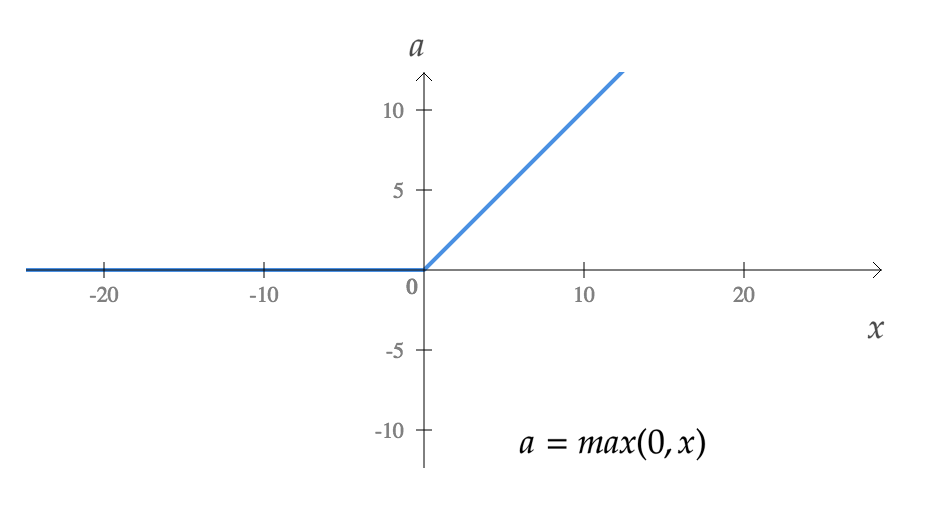
\includegraphics[width=0.45\linewidth , height=0.30\linewidth]{images/relu.png}}
\subcaptionbox{\label{sfig:sigmoid}}{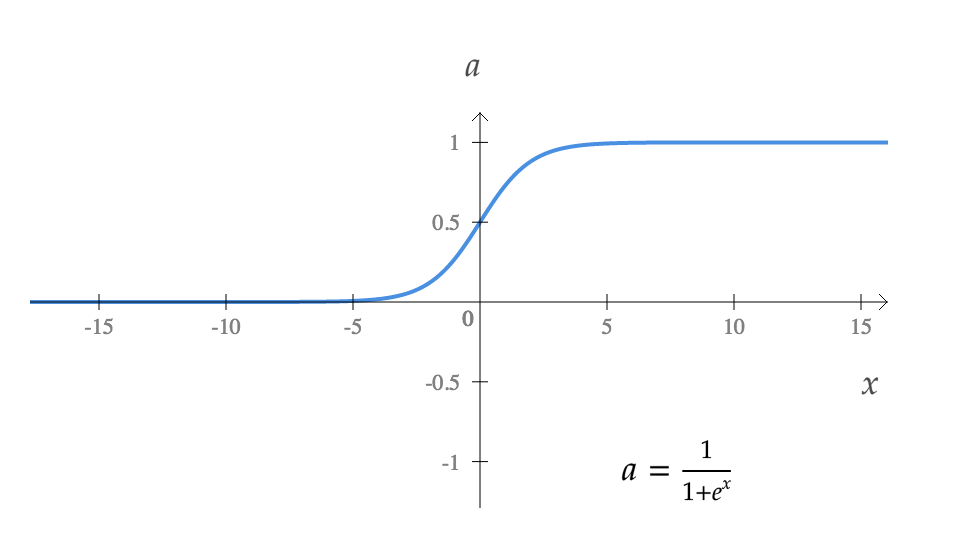
\includegraphics[width=0.45\linewidth , height=0.30\linewidth]{images/sigmoid.png}}
\caption{Common choices of activation functions:~\subref{sfig:relu} Relu function $a=max(0,x)$ (simply cutting values below zero) and ~\subref{sfig:sigmoid} Sigmoid function $a=\frac{1}{1+e^{x}}$, which forces the values to be between zero and one.}
\label{fig:activation}
\end{figure}
\subsection{Training  Neural networks}
Consider the output $\hat { y } $ as the prediction of our network for some task. In a supervised learning problem the aim is to reduce the error between the prediction ($\hat { y } $) and the true label $y$. As a result the cost function can be defined as $J$ in Equation~\ref{eq:cost_nn}, where $L$ denotes the loss function on a single training example and $m$ is the size of the training set. The cost function is simply the sum of all losses on the training set.
\begin{equation}
J(\theta,b)=\sum _{ j=1 }^{ m }{ L( } \hat { y }^{ (i) } ,y^{ (i) })
\label{eq:cost_nn}
\end{equation}
The goal of the training phase is to learn $\theta$ and $b$ such that the overall cost is minimized. \\
\noindent 
One method to solve this optimization problem is called \emph{Gradient Descent} (GD)~\brackettext{\cite{DBLP:journals/corr/Ruder16}}. Considering the most simple case (a function with only one parameter) the gradient descent is illustrated in Figure~\ref{fig:gradientD}. Gradient descent is a way to minimize an objective function parameterized by a model’s parameters by updating the parameters in the opposite direction of the gradient w.r.t. to the parameters. The algorithm for one parameter $\theta$ can be
seen in Algorithm~\ref{algo:gd}, $\alpha$ is the \emph{learning rate} or the step size and shows how big a step we take in each iteration. As shown in Figure~\ref{fig:gradientD} the derivative or the slope of the function is positive on the right side of the minimum (the update rule will decrease $\theta$) and negative on the left size (the update rule will increase $\theta$). \\


\begin{algorithm}[htbp]
  %
  \begin{algorithmic}[1]
    \newcommand{\UF}{\mathrm{U}}
   \While{(not converged)}
 \State $\theta=: \theta- \alpha\frac { \partial J(\theta) }{ \partial \theta } $
  \EndWhile
  \end{algorithmic}
  %
\caption{:Gradient decent }
 \label{algo:gd}
\end{algorithm}

\begin{figure}
\centering 
\resizebox{0.65\textwidth}{0.4\textwidth}{      
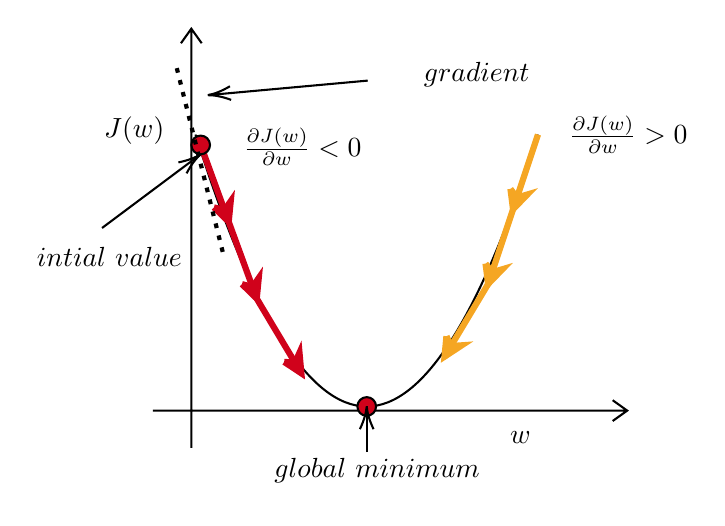
\begin{tikzpicture}[x=0.75pt,y=0.75pt,yscale=-1,xscale=1]
%uncomment if require: \path (0,300); %set diagram left start at 0, and has height of 300

\draw  (75,190) -- (303.5,190)(93.5,6) -- (93.5,208) (296.5,185) -- (303.5,190) -- (296.5,195) (88.5,13) -- (93.5,6) -- (98.5,13)  ;
\draw   (95.5,57) .. controls (150.5,231.67) and (205.5,231.67) .. (260.5,57) ;
\draw [color={rgb, 255:red, 208; green, 2; blue, 27 }  ,draw opacity=1 ][line width=2.25]    (98,62) -- (111.5,99) ;
\draw [shift={(111.5,99)}, rotate = 249.95] [color={rgb, 255:red, 208; green, 2; blue, 27 }  ,draw opacity=1 ][fill={rgb, 255:red, 208; green, 2; blue, 27 }  ,fill opacity=1 ][line width=2.25]   (8.93,-4.29) -- (0,0) -- (8.93,4.29) -- (5.93,0) -- (8.93,-4.29)    ;

\draw [color={rgb, 255:red, 208; green, 2; blue, 27 }  ,draw opacity=1 ][line width=2.25]    (111.5,99) -- (125,136) ;
\draw [shift={(125,136)}, rotate = 249.95] [color={rgb, 255:red, 208; green, 2; blue, 27 }  ,draw opacity=1 ][fill={rgb, 255:red, 208; green, 2; blue, 27 }  ,fill opacity=1 ][line width=2.25]   (8.93,-4.29) -- (0,0) -- (8.93,4.29) -- (5.93,0) -- (8.93,-4.29)    ;

\draw [color={rgb, 255:red, 208; green, 2; blue, 27 }  ,draw opacity=1 ][line width=2.25]    (125,136) -- (146.5,172) ;
\draw [shift={(146.5,172)}, rotate = 239.15] [color={rgb, 255:red, 208; green, 2; blue, 27 }  ,draw opacity=1 ][fill={rgb, 255:red, 208; green, 2; blue, 27 }  ,fill opacity=1 ][line width=2.25]   (8.93,-4.29) -- (0,0) -- (8.93,4.29) -- (5.93,0) -- (8.93,-4.29)    ;

\draw [color={rgb, 255:red, 245; green, 166; blue, 35 }  ,draw opacity=1 ][line width=2.25]    (260.5,57) -- (248.5,93) ;
\draw [shift={(248.5,93)}, rotate = 288.43] [color={rgb, 255:red, 245; green, 166; blue, 35 }  ,draw opacity=1 ][fill={rgb, 255:red, 245; green, 166; blue, 35 }  ,fill opacity=1 ][line width=2.25]   (8.93,-4.29) -- (0,0) -- (8.93,4.29) -- (5.93,0) -- (8.93,-4.29)    ;

\draw [color={rgb, 255:red, 245; green, 166; blue, 35 }  ,draw opacity=1 ][line width=2.25]    (248.5,93) -- (236.5,129) ;
\draw [shift={(236.5,129)}, rotate = 288.43] [color={rgb, 255:red, 245; green, 166; blue, 35 }  ,draw opacity=1 ][fill={rgb, 255:red, 245; green, 166; blue, 35 }  ,fill opacity=1 ][line width=2.25]   (8.93,-4.29) -- (0,0) -- (8.93,4.29) -- (5.93,0) -- (8.93,-4.29)    ;

\draw [color={rgb, 255:red, 245; green, 166; blue, 35 }  ,draw opacity=1 ][line width=2.25]    (236.5,129) -- (215.5,164) ;
\draw [shift={(215.5,164)}, rotate = 300.96] [color={rgb, 255:red, 245; green, 166; blue, 35 }  ,draw opacity=1 ][fill={rgb, 255:red, 245; green, 166; blue, 35 }  ,fill opacity=1 ][line width=2.25]   (8.93,-4.29) -- (0,0) -- (8.93,4.29) -- (5.93,0) -- (8.93,-4.29)    ;

\draw  [fill={rgb, 255:red, 208; green, 2; blue, 27 }  ,fill opacity=1 ]  (98, 62) circle [x radius= 4.5, y radius= 4.5]  ;
\draw    (50.5,102) -- (98,66.5) ;
\draw [shift={(98,66.5)}, rotate = 503.23] [color={rgb, 255:red, 0; green, 0; blue, 0 }  ]   (0,0) .. controls (3.31,-0.3) and (6.95,-1.4) .. (10.93,-3.29)(0,0) .. controls (3.31,0.3) and (6.95,1.4) .. (10.93,3.29)   ;

\draw  [fill={rgb, 255:red, 208; green, 2; blue, 27 }  ,fill opacity=1 ]  (178, 188) circle [x radius= 4.5, y radius= 4.5]  ;
\draw    (178,210) -- (178,188) ;
\draw [shift={(178,188)}, rotate = 450] [color={rgb, 255:red, 0; green, 0; blue, 0 }  ]   (0,0) .. controls (3.31,-0.3) and (6.95,-1.4) .. (10.93,-3.29)(0,0) .. controls (3.31,0.3) and (6.95,1.4) .. (10.93,3.29)   ;

\draw [line width=1.5]  [dash pattern={on 1.69pt off 2.76pt}]  (86.5,25) -- (109.5,117) ;


\draw    (178.5,31) -- (101.5,38) ;
\draw [shift={(101.5,38)}, rotate = 354.81] [color={rgb, 255:red, 0; green, 0; blue, 0 }  ]   (0,0) .. controls (3.31,-0.3) and (6.95,-1.4) .. (10.93,-3.29)(0,0) .. controls (3.31,0.3) and (6.95,1.4) .. (10.93,3.29)   ;


\draw (252,203) node   {$w$};
\draw (66,55) node   {$J( w)$};
\draw (147,63) node   {$\frac{\partial J( w)}{\partial w} < 0$};
\draw (304,57) node   {$\frac{\partial J( w)}{\partial w}  >0$};
\draw (183,219) node   {$global\ minimum$};
\draw (54,116) node   {$intial\ value$};
\draw (231,28) node   {$gradient$};


\end{tikzpicture}

}
\caption{Gradient decent on a function with only one parameter. In each iteration, we take a step in the direction of the gradient. The gradient will guide the algorithm to the functions minimum. }
\label{fig:gradientD}
\end{figure}
\noindent
In a dataset with $m$ training examples, for each training example, the partial derivative of the cost function with respect to every weight and bias has to be calculated and accumulated. After iterating through all the training examples the weights and bias term will be updated according to Algorithm~\ref{algo:gd}. This process is repeated from start to finish for some number of iterations. There exist three main variations of~GD: 
\begin{itemize}
\item \textbf{Mini-batch GD: } Instead of iterating over all training examples, a subset of a batch is considered, before making an update. This is a good choice for very large datasets.
\item \textbf{Stochastic-GD: } In this case, only one example is looked at, before making an update. 
\item \textbf{Batch-GD: } The original algorithm with iteration over all examples. 
\end{itemize}

\subsection{Embeddings}\label{subsec:embeddings}
One of the challenges of machine learning is to come up with valuable features for algorithms. These features often have to be task specific and reflect the needs of the downstream tasks(a task that uses embeddings as input featues). \emph{Representation learning} attempts to learn good features and representations automatically~\brackettext{\cite{SCHOL:journals/FDS/ZhongWD16}}. PCA is one example of traditional methods for learning low-dimensional representation from high dimensional data. In a deep learning architecture, the output of each intermediate layer can be viewed as a representation of the original input data. As illustrated in Figure~\ref{fig:preceptron} each unit of the network computes a non-linear combination of the inputs which is used by the next layer. If the dimension of the hidden layer is much smaller than the input layer, a low dimensional representation of the data is learned in the hidden layer. Based on this principle almost any data can be transformed into an embedding with lower dimensions. In this work we focus on only two types, namely, \emph{word embeddings} and  \emph{graph embeddings} \\
\noindent
Word embeddings try to learn dense vector representation for each word in the text. The text is inherently high dimensional. In most traditional NLP systems, each word is represented as a one-hot vector~\footnote{binary vector in the size of the vocabulary that has the value of one on the index of the word it refers to and zeroes in all other indexes.} of size equal to the size of the vocabulary, which is not only sparse but high dimensional. By feeding these high dimensional representations to a neural network with a smaller hidden layer, a new representation (usually in the order of $100$ dimensions) of each word can be learned. Although neural networks can be used in supervised and unsupervised learning, generally, the embedding is learned to form a supervised learning problem. For this purpose, different models have been proposed, the most famous being word2vec. All the models follow the same principle illustrated in Figure~\ref{fig:emb}. The size of the output layer depends on the particular architecture and the cost function. In addition, the network can composed of multiple layers, but for our purposes, we focus on shallow networks with only one hidden layer. In Section~\ref{sec:wordembeddig}, we will discuss GloVe and word2vec in more details. \\
\noindent
Graph embedding tries to convert a high dimensional graph with edges and nodes, into a low dimensional space while preserving the graph information. Graphs are complex and contain many attributes. Therefore, transforming them into low dimensional spaces is not a trivial task. There are various methods to embed nodes, edges or whole-graph. For the purpose of this study, we focus on \emph{node embeddings}, which represents each node as a vector in a low dimensional space. Nodes that are \emph{``close"} in the graph should be closer in the new space. The difference between various techniques lies in how they define the  \emph{``closeness"}~\brackettext{\cite{DBLP:journals/tkde/CaiZC18}}. In the next section, we will give a brief introduction into co-occurrence graphs and in Section~\ref{sec:graph} the well-known graph embedding methods are explained.  
\begin{figure}
\centering 
\resizebox{0.8\textwidth}{0.48\textwidth}{      
\begin{tikzpicture}[x=0.75pt,y=0.75pt,yscale=-1,xscale=1]
%uncomment if require: \path (0,406); %set diagram left start at 0, and has height of 406

\draw  [color={rgb, 255:red, 208; green, 2; blue, 27 }  ,draw opacity=1 ]  (302, 69) circle [x radius= 25, y radius= 25]  ;
\draw  [color={rgb, 255:red, 208; green, 2; blue, 27 }  ,draw opacity=1 ]  (301, 135) circle [x radius= 25, y radius= 25]  ;
\draw  [color={rgb, 255:red, 208; green, 2; blue, 27 }  ,draw opacity=1 ]  (301, 200) circle [x radius= 25, y radius= 25]  ;
\draw    (322.5,79) -- (411.5,133) ;
\draw [shift={(411.5,133)}, rotate = 211.25] [color={rgb, 255:red, 0; green, 0; blue, 0 }  ]   (0,0) .. controls (3.31,-0.3) and (6.95,-1.4) .. (10.93,-3.29)(0,0) .. controls (3.31,0.3) and (6.95,1.4) .. (10.93,3.29)   ;

\draw    (326,135) -- (411.5,133) ;
\draw [shift={(411.5,133)}, rotate = 538.6600000000001] [color={rgb, 255:red, 0; green, 0; blue, 0 }  ]   (0,0) .. controls (3.31,-0.3) and (6.95,-1.4) .. (10.93,-3.29)(0,0) .. controls (3.31,0.3) and (6.95,1.4) .. (10.93,3.29)   ;

\draw    (326,200) -- (411.5,133) ;
\draw [shift={(411.5,133)}, rotate = 501.92] [color={rgb, 255:red, 0; green, 0; blue, 0 }  ]   (0,0) .. controls (3.31,-0.3) and (6.95,-1.4) .. (10.93,-3.29)(0,0) .. controls (3.31,0.3) and (6.95,1.4) .. (10.93,3.29)   ;

\draw  [color={rgb, 255:red, 208; green, 2; blue, 27 }  ,draw opacity=1 ]  (433, 69) circle [x radius= 25, y radius= 25]  ;
\draw    (477.5,183) -- (551.5,183) ;
\draw [shift={(551.5,183)}, rotate = 180] [color={rgb, 255:red, 0; green, 0; blue, 0 }  ]   (0,0) .. controls (3.31,-0.3) and (6.95,-1.4) .. (10.93,-3.29)(0,0) .. controls (3.31,0.3) and (6.95,1.4) .. (10.93,3.29)   ;

\draw    (165.43, 104) circle [x radius= 25, y radius= 25]  ;
\draw    (168, 177) circle [x radius= 25, y radius= 25]  ;
\draw    (175, 256) circle [x radius= 25, y radius= 25]  ;
\draw    (164.19, 34.33) circle [x radius= 25.19, y radius= 25.19]  ;
\draw    (188.38,44.33) -- (279,75) ;
\draw [shift={(279,75)}, rotate = 198.7] [color={rgb, 255:red, 0; green, 0; blue, 0 }  ]   (0,0) .. controls (3.31,-0.3) and (6.95,-1.4) .. (10.93,-3.29)(0,0) .. controls (3.31,0.3) and (6.95,1.4) .. (10.93,3.29)   ;

\draw    (188.38,44.33) -- (279,142) ;
\draw [shift={(279,142)}, rotate = 227.14] [color={rgb, 255:red, 0; green, 0; blue, 0 }  ]   (0,0) .. controls (3.31,-0.3) and (6.95,-1.4) .. (10.93,-3.29)(0,0) .. controls (3.31,0.3) and (6.95,1.4) .. (10.93,3.29)   ;

\draw    (188.38,44.33) -- (279,207) ;
\draw [shift={(279,207)}, rotate = 240.88] [color={rgb, 255:red, 0; green, 0; blue, 0 }  ]   (0,0) .. controls (3.31,-0.3) and (6.95,-1.4) .. (10.93,-3.29)(0,0) .. controls (3.31,0.3) and (6.95,1.4) .. (10.93,3.29)   ;

\draw    (189.43,106) -- (279,207) ;
\draw [shift={(279,207)}, rotate = 228.43] [color={rgb, 255:red, 0; green, 0; blue, 0 }  ]   (0,0) .. controls (3.31,-0.3) and (6.95,-1.4) .. (10.93,-3.29)(0,0) .. controls (3.31,0.3) and (6.95,1.4) .. (10.93,3.29)   ;

\draw    (189.43,106) -- (279,142) ;
\draw [shift={(279,142)}, rotate = 201.9] [color={rgb, 255:red, 0; green, 0; blue, 0 }  ]   (0,0) .. controls (3.31,-0.3) and (6.95,-1.4) .. (10.93,-3.29)(0,0) .. controls (3.31,0.3) and (6.95,1.4) .. (10.93,3.29)   ;

\draw    (189.43,106) -- (279,75) ;
\draw [shift={(279,75)}, rotate = 520.9100000000001] [color={rgb, 255:red, 0; green, 0; blue, 0 }  ]   (0,0) .. controls (3.31,-0.3) and (6.95,-1.4) .. (10.93,-3.29)(0,0) .. controls (3.31,0.3) and (6.95,1.4) .. (10.93,3.29)   ;

\draw    (191,168) -- (279,75) ;
\draw [shift={(279,75)}, rotate = 493.42] [color={rgb, 255:red, 0; green, 0; blue, 0 }  ]   (0,0) .. controls (3.31,-0.3) and (6.95,-1.4) .. (10.93,-3.29)(0,0) .. controls (3.31,0.3) and (6.95,1.4) .. (10.93,3.29)   ;

\draw    (191,168) -- (279,142) ;
\draw [shift={(279,142)}, rotate = 523.54] [color={rgb, 255:red, 0; green, 0; blue, 0 }  ]   (0,0) .. controls (3.31,-0.3) and (6.95,-1.4) .. (10.93,-3.29)(0,0) .. controls (3.31,0.3) and (6.95,1.4) .. (10.93,3.29)   ;

\draw    (191,168) -- (279,207) ;
\draw [shift={(279,207)}, rotate = 203.9] [color={rgb, 255:red, 0; green, 0; blue, 0 }  ]   (0,0) .. controls (3.31,-0.3) and (6.95,-1.4) .. (10.93,-3.29)(0,0) .. controls (3.31,0.3) and (6.95,1.4) .. (10.93,3.29)   ;

\draw    (190,233) -- (279,75) ;
\draw [shift={(279,75)}, rotate = 479.39] [color={rgb, 255:red, 0; green, 0; blue, 0 }  ]   (0,0) .. controls (3.31,-0.3) and (6.95,-1.4) .. (10.93,-3.29)(0,0) .. controls (3.31,0.3) and (6.95,1.4) .. (10.93,3.29)   ;

\draw    (190,233) -- (279,142) ;
\draw [shift={(279,142)}, rotate = 494.36] [color={rgb, 255:red, 0; green, 0; blue, 0 }  ]   (0,0) .. controls (3.31,-0.3) and (6.95,-1.4) .. (10.93,-3.29)(0,0) .. controls (3.31,0.3) and (6.95,1.4) .. (10.93,3.29)   ;

\draw    (190,233) -- (279,207) ;
\draw [shift={(279,207)}, rotate = 523.72] [color={rgb, 255:red, 0; green, 0; blue, 0 }  ]   (0,0) .. controls (3.31,-0.3) and (6.95,-1.4) .. (10.93,-3.29)(0,0) .. controls (3.31,0.3) and (6.95,1.4) .. (10.93,3.29)   ;

\draw   (149.5,289) .. controls (149.5,293.67) and (151.83,296) .. (156.5,296) -- (172,296) .. controls (178.67,296) and (182,298.33) .. (182,303) .. controls (182,298.33) and (185.33,296) .. (192,296)(189,296) -- (207.5,296) .. controls (212.17,296) and (214.5,293.67) .. (214.5,289) ;
\draw   (267,233) .. controls (266.89,237.67) and (269.17,240.05) .. (273.84,240.16) -- (301.1,240.77) .. controls (307.76,240.92) and (311.04,243.32) .. (310.93,247.99) .. controls (311.04,243.32) and (314.42,241.07) .. (321.09,241.22)(318.09,241.15) -- (348.34,241.83) .. controls (353.01,241.94) and (355.39,239.66) .. (355.5,234.99) ;
\draw   (397,302) .. controls (396.89,306.67) and (399.17,309.05) .. (403.84,309.16) -- (431.1,309.77) .. controls (437.76,309.92) and (441.04,312.32) .. (440.93,316.99) .. controls (441.04,312.32) and (444.42,310.07) .. (451.09,310.22)(448.09,310.15) -- (478.34,310.83) .. controls (483.01,310.94) and (485.39,308.66) .. (485.5,303.99) ;
\draw    (7, 87) rectangle (137.5, 111.33)   ;
\draw    (7, 181) rectangle (137.5, 205.33)   ;
\draw    (8, 270) rectangle (138.5, 294.33)   ;
\draw  [color={rgb, 255:red, 208; green, 2; blue, 27 }  ,draw opacity=1 ]  (432, 143) circle [x radius= 25, y radius= 25]  ;
\draw  [color={rgb, 255:red, 208; green, 2; blue, 27 }  ,draw opacity=1 ]  (435, 207) circle [x radius= 25, y radius= 25]  ;
\draw  [color={rgb, 255:red, 208; green, 2; blue, 27 }  ,draw opacity=1 ]  (437, 272) circle [x radius= 25, y radius= 25]  ;
\draw    (326,135) -- (410,207) ;
\draw [shift={(410,207)}, rotate = 220.6] [color={rgb, 255:red, 0; green, 0; blue, 0 }  ]   (0,0) .. controls (3.31,-0.3) and (6.95,-1.4) .. (10.93,-3.29)(0,0) .. controls (3.31,0.3) and (6.95,1.4) .. (10.93,3.29)   ;

\draw    (322.5,79) -- (408,69) ;
\draw [shift={(408,69)}, rotate = 533.3299999999999] [color={rgb, 255:red, 0; green, 0; blue, 0 }  ]   (0,0) .. controls (3.31,-0.3) and (6.95,-1.4) .. (10.93,-3.29)(0,0) .. controls (3.31,0.3) and (6.95,1.4) .. (10.93,3.29)   ;

\draw    (322.5,79) -- (410,207) ;
\draw [shift={(410,207)}, rotate = 235.64] [color={rgb, 255:red, 0; green, 0; blue, 0 }  ]   (0,0) .. controls (3.31,-0.3) and (6.95,-1.4) .. (10.93,-3.29)(0,0) .. controls (3.31,0.3) and (6.95,1.4) .. (10.93,3.29)   ;

\draw    (322.5,79) -- (412,272) ;
\draw [shift={(412,272)}, rotate = 245.12] [color={rgb, 255:red, 0; green, 0; blue, 0 }  ]   (0,0) .. controls (3.31,-0.3) and (6.95,-1.4) .. (10.93,-3.29)(0,0) .. controls (3.31,0.3) and (6.95,1.4) .. (10.93,3.29)   ;

\draw    (326,135) -- (408,69) ;
\draw [shift={(408,69)}, rotate = 501.17] [color={rgb, 255:red, 0; green, 0; blue, 0 }  ]   (0,0) .. controls (3.31,-0.3) and (6.95,-1.4) .. (10.93,-3.29)(0,0) .. controls (3.31,0.3) and (6.95,1.4) .. (10.93,3.29)   ;

\draw    (326,200) -- (410,207) ;
\draw [shift={(410,207)}, rotate = 184.76] [color={rgb, 255:red, 0; green, 0; blue, 0 }  ]   (0,0) .. controls (3.31,-0.3) and (6.95,-1.4) .. (10.93,-3.29)(0,0) .. controls (3.31,0.3) and (6.95,1.4) .. (10.93,3.29)   ;

\draw    (326,200) -- (408,69) ;
\draw [shift={(408,69)}, rotate = 482.04] [color={rgb, 255:red, 0; green, 0; blue, 0 }  ]   (0,0) .. controls (3.31,-0.3) and (6.95,-1.4) .. (10.93,-3.29)(0,0) .. controls (3.31,0.3) and (6.95,1.4) .. (10.93,3.29)   ;

\draw    (328,200) -- (412,272) ;
\draw [shift={(412,272)}, rotate = 220.6] [color={rgb, 255:red, 0; green, 0; blue, 0 }  ]   (0,0) .. controls (3.31,-0.3) and (6.95,-1.4) .. (10.93,-3.29)(0,0) .. controls (3.31,0.3) and (6.95,1.4) .. (10.93,3.29)   ;

\draw    (326,135) -- (412,272) ;
\draw [shift={(412,272)}, rotate = 237.88] [color={rgb, 255:red, 0; green, 0; blue, 0 }  ]   (0,0) .. controls (3.31,-0.3) and (6.95,-1.4) .. (10.93,-3.29)(0,0) .. controls (3.31,0.3) and (6.95,1.4) .. (10.93,3.29)   ;


\draw (303.21,68.84) node [color={rgb, 255:red, 208; green, 2; blue, 27 }  ,opacity=1 ]  {$a^{( 2)}_{1}$};
\draw (305.21,136.84) node [color={rgb, 255:red, 208; green, 2; blue, 27 }  ,opacity=1 ]  {$a^{( 2)}_{2}$};
\draw (302.21,203.84) node [color={rgb, 255:red, 208; green, 2; blue, 27 }  ,opacity=1 ]  {$a^{( 2)}_{3}$};
\draw (169,178) node   {$x_{2}$};
\draw (168.37,102.96) node   {$x_{1}$};
\draw (175,256) node   {$x_{3}$};
\draw (167.21,32.84) node   {$1$};
\draw (578,186) node   {$\hat{y}$};
\draw (183,326) node   {$input\ layer$};
\draw (315,272) node   {$ \begin{gathered}
low\ dimensional\ \\
representation
\end{gathered}$};
\draw (444,335) node   {$output\ layer$};
\draw (72,99) node   {$0\ \ 0\ \ 0\ \ 0\ \ 0\ \ 0\ \ ..\ 0$};
\draw (13,77) node [rotate=-270]  {$a$};
\draw (29,60) node [rotate=-270]  {$brown$};
\draw (46,63) node [rotate=-270]  {$dog$};
\draw (78,63) node [rotate=-270]  {$jumps$};
\draw (129,62) node [rotate=-270]  {$zoo$};
\draw (64,65) node [rotate=-270]  {$fox$};
\draw (72,193) node   {$0\ \ 0\ \ 0\ \ 1\ \ 0\ \ 0\ ..\ 0$};
\draw (13,171) node [rotate=-270]  {$a$};
\draw (29,154) node [rotate=-270]  {$brown$};
\draw (46,157) node [rotate=-270]  {$dog$};
\draw (78,157) node [rotate=-270]  {$jumps$};
\draw (64,159) node [rotate=-270]  {$fox$};
\draw (73,282) node   {$0\ \ 0\ \ 0\ \ 0\ \ 0\ \ 0\ \ ..\ 0$};
\draw (14,260) node [rotate=-270]  {$a$};
\draw (30,243) node [rotate=-270]  {$brown$};
\draw (47,246) node [rotate=-270]  {$dog$};
\draw (79,246) node [rotate=-270]  {$jumps$};
\draw (65,248) node [rotate=-270]  {$fox$};
\draw (125,159) node [rotate=-270]  {$zoo$};
\draw (130,246) node [rotate=-270]  {$zoo$};
\draw (110,64) node   {$...$};
\draw (108,160) node   {$...$};
\draw (111,248) node   {$...$};


\end{tikzpicture}

}
\caption{Underlying principle of word embeddings. The high dimensional one-hot vectors are the input of the network, through the hidden layer a dense representation is learned to either predict the surrounding words or optimize a different cost function in the output layer.}
\label{fig:emb}
\end{figure}

\section{Co-occurrence Graphs}
\label{sec:graph}
Co-occurrence analysis, in terms of graphs, is not limited to text mining but is a tool to find potential relationships between people, organizations, concepts, and biological organisms.~\brackettext{\cite{SCHOL:journal/NAR/shiri}}. A word co-occurrence graph shows the word interactions in a corpus. A co-occurrence graph $G=(T,E)$ is defined by a set of terms $T$ as nodes and edges $E$ between them, where there is an edge based on their paired presence in a unit of text. If the entities in the text are annotated, the graph shows the relationship between entities and terms that occur in the text. There is an edge between two words, if they occur in the same sentence or paragraph~\brackettext{\cite{DBLP:conf/interspeech/YinBB18}}. If the graph is weighted, the edges indicate the strength of
the connection between two words or entities, which related to the number of their co-occurrences or some kind of distance measure, e.g., number of tokens between them.~\brackettext{\cite{SCHOL:book/mihalcea2011}}. Since these graphs encode all important words in the vocabulary, they can form a graph-based representation of the corpus, which we use instead of a textual corpus to generate embeddings, where relations between nearby words can be extracted based on edges and nearby nodes.

\emph{LOAD: Implicit Graph of Entities:} The LOAD~\brackettext{\cite{DBLP:conf/sigir/SpitzG16}} model is an entity co-occurrence graph representation of large document collections. For each document, named entities from sentences are extracted and connected based on their distance in a graph structure. The original LOAD model contains node types of pages and Sentences as well, which we disregard for the creation of faceted embeddings. \\
Equation~\ref{eq:load_dist} shows the weighing of a single edge in the LOAD model between two entities $v$ and $s$, where $\delta $ is a distance function. $\delta $ equals the number of sentences between the
instances, or $0$ if they occur in the same sentence. If $i$ and$ j$
do not occur on the same page: $ \delta(i, j) := \inf$. $ I_{ v }$ and $I_{ s } $ are the set of all instances of $v$ and $s$ in the corpus. $exp$ forces the weight to diminish exponentially with the distance. Eventually, the sum of all these exponential distances creates the final weight. 
\begin{equation}
e (v,s)\quad =\quad \sum _{ i\in I_{ v } \\ j\in I_{ s } }^{  }{ exp } (-\delta (i,j))
\label{eq:load_dist}
\end{equation}
The weights generated in this way encode the importance of one entity to another. The distance decays as the number of sentences between two entities grows.  In addition, long-distance connections are considered very weak and are cut-off.  However, terms are less likely to be related to entities outside of their own sentence, so the edges between terms and entities are limited to those that appear in the same sentence~\brackettext{\cite{DBLP:conf/sigir/SpitzG16}}. 

\section{Word Embeddings }
\label{sec:wordembeddig}
A word embedding is defined as a mapping $ V\rightarrow { R }^{ d }:v \rightarrow w $ that maps a word $v$ from a vocabulary $V$ to a vector  $w$  in an embedding space of dimensionality $d$ ~\brackettext{\cite{DBLP:conf/emnlp/SchnabelLMJ15}}. \\
The first model to learn word embeddings as dense vector was presented by~\brackettext{\cite{DBLP:conf/nips/BengioDV00}}, in which a feature vector, much smaller than the size of the vocabulary, was used to express words using a probabilistic model. The work of~\brackettext{\cite{DBLP:journals/jmlr/CollobertWBKKK11}} proved that word representation could not only be achieved through probabilistic models, but that neural network architectures can also learn these internal representations from vast amounts of mostly unlabeled training data. However, it was not until word2vec~\brackettext{\cite{DBLP:journals/corr/abs-1301-3781}} that word embeddings became applicable to large corpora. 
Window-based models such as word2vec learn the embeddings in terms of a supervised learning task, where the objective is to predict a word's context given a center word in a fixed window. A noticeable disadvantage of these models is that they do not operate directly on the co-occurrence statistics of the corpus. Instead, they scan context windows across sentences, which fails to take advantage of the vast amount of repetition in the data. Regardless of the fact that many words co-occur multiple time, for multiple passes through the data, a window-based method has to parse the whole corpus several times. On the other hand, a co-occurrence matrix can capture this repetition in a compact way and hence, save time and computational power.  \\
In contrast, matrix factorization methods operate directly on the co-occurrence matrix and capture the full statistics. Before word2vec, similar embeddings were generated using \emph{Singular Value Decomposition} (SVD) on co-occurrence matrices and keeping the top \emph{k} dimensions. These methods were also able to capture many semantic and syntactic analogies~\brackettext{\cite{SCHOL:journals/acm/Rohde}}. \brackettext{\cite{DBLP:conf/nips/LevyG14}} showed that implicitly factorizing
a word-context matrix, whose cells are the \emph{Point-wise Mutual Information} (PMI) of
the respective word and context pairs, can generate embeddings close to word2vec. The main disadvantage of count based methods is that they are computationally slow on large matrices. In addition, adding new words to the model is difficult, since it requires training a new model from the start.\\
The GloVe~\brackettext{\cite{DBLP:conf/emnlp/PenningtonSM14}} model combines the matrix factorization for generating embeddings with window-based methods and uses the global statistics of the corpus or in another word the co-occurrence matrix to generate embeddings. In addition, unlike the word2vec model that scales with the size of the corpus, general statistics of the data has to be generated only once in terms of the co-occurrence matrix and then additional computations can be performed on matrix alone.
\subsection{Word2vec: Distributed Representations of Words }
\label{subsec:word2vec}
\begin{figure}
\centering 
\resizebox{0.63\textwidth}{0.5\textwidth}{      
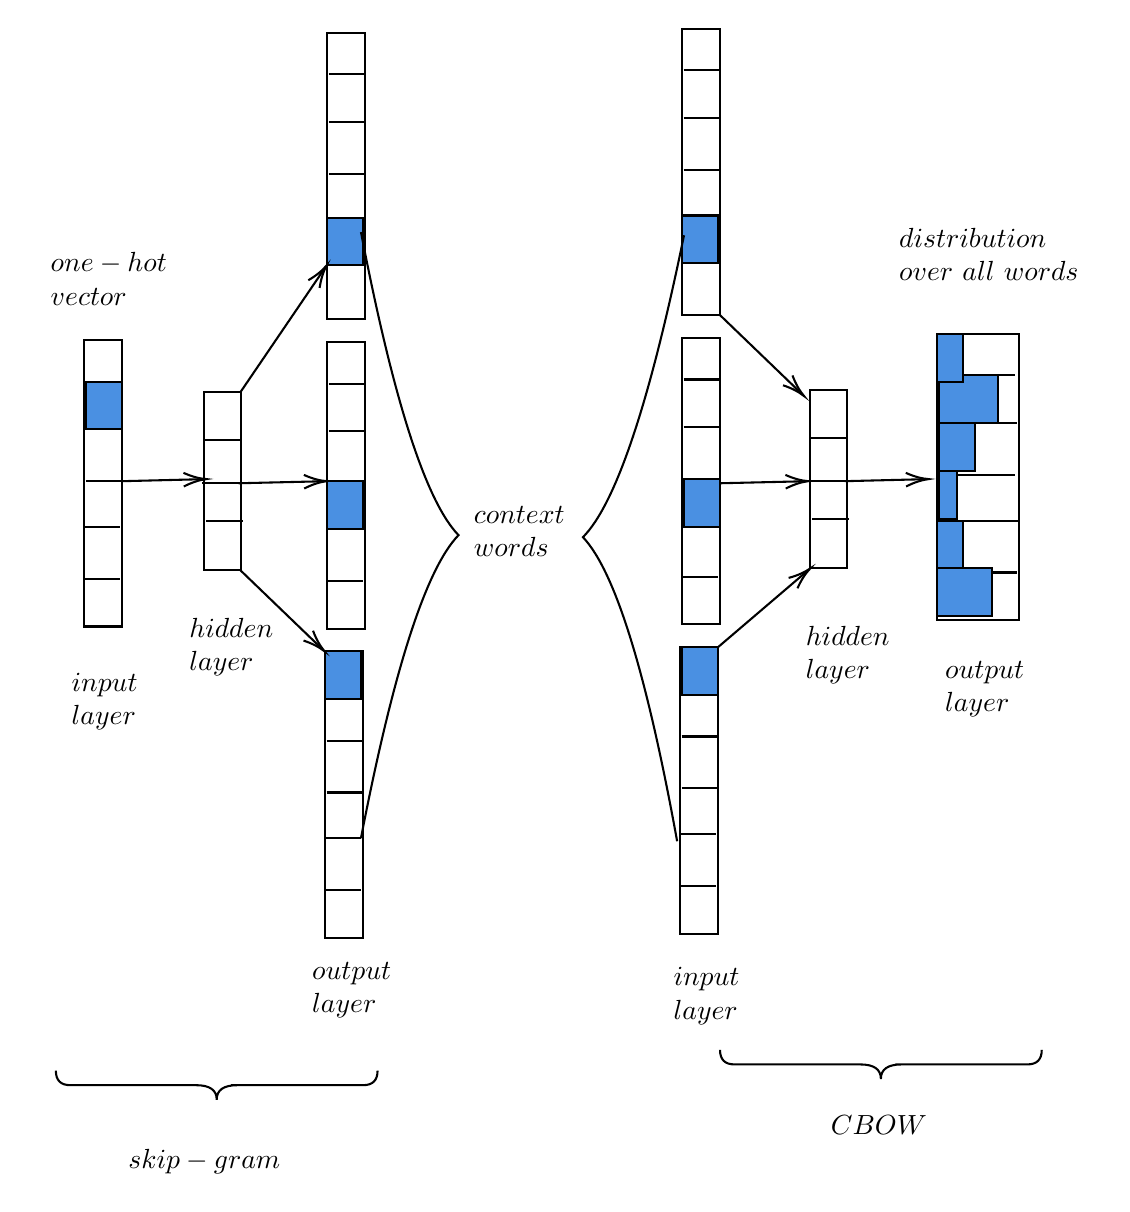
\begin{tikzpicture}[x=0.75pt,y=0.75pt,yscale=-1,xscale=1]
%uncomment if require: \path (0,608); %set diagram left start at 0, and has height of 608

%Shape: Rectangle [id:dp3485846016801524] 
\draw   (32,156) -- (50.5,156) -- (50.5,294) -- (32,294) -- cycle ;
%Shape: Rectangle [id:dp8456709052048703] 
\draw   (90,181) -- (107.5,181) -- (107.5,267) -- (90,267) -- cycle ;
%Straight Lines [id:da261980941990962] 
\draw    (33,176) -- (50.5,176) ;


%Straight Lines [id:da2112077987204617] 
\draw    (33,199) -- (50.5,199) ;


%Straight Lines [id:da8306488203565181] 
\draw    (33,224) -- (50.5,224) ;


%Straight Lines [id:da2601610712460867] 
\draw    (32,246) -- (49.5,246) ;


%Straight Lines [id:da5238964279791503] 
\draw    (32,271) -- (49.5,271) ;


%Straight Lines [id:da8696264510823728] 
\draw    (90,204) -- (107.5,204) ;


%Straight Lines [id:da18281681508420422] 
\draw    (89,225) -- (106.5,225) ;


%Straight Lines [id:da7605537343893694] 
\draw    (91,243) -- (108.5,243) ;


%Shape: Rectangle [id:dp7179646823512316] 
\draw   (149,8) -- (167.5,8) -- (167.5,146) -- (149,146) -- cycle ;
%Straight Lines [id:da37315938965868667] 
\draw    (150,28) -- (167.5,28) ;


%Straight Lines [id:da17887383176459348] 
\draw    (150,51) -- (167.5,51) ;


%Straight Lines [id:da05916336325961158] 
\draw    (150,76) -- (167.5,76) ;


%Straight Lines [id:da5760610647676259] 
\draw    (149,98) -- (166.5,98) ;


%Straight Lines [id:da6528261772940696] 
\draw    (149,120) -- (166.5,120) ;


%Shape: Rectangle [id:dp8883127519205649] 
\draw   (149,157) -- (167.5,157) -- (167.5,295) -- (149,295) -- cycle ;
%Straight Lines [id:da06170003747009711] 
\draw    (150,177) -- (167.5,177) ;


%Straight Lines [id:da41536185218273225] 
\draw    (150,200) -- (167.5,200) ;


%Straight Lines [id:da42678869727576263] 
\draw    (150,225) -- (167.5,225) ;


%Straight Lines [id:da4310051753333286] 
\draw    (149,247) -- (166.5,247) ;


%Straight Lines [id:da053035267754805604] 
\draw    (149,272) -- (166.5,272) ;


%Shape: Rectangle [id:dp5517809725941882] 
\draw   (148,306) -- (166.5,306) -- (166.5,444) -- (148,444) -- cycle ;
%Straight Lines [id:da4185941337540897] 
\draw    (149,326) -- (166.5,326) ;


%Straight Lines [id:da47456328490948096] 
\draw    (149,349) -- (166.5,349) ;


%Straight Lines [id:da5901537425032239] 
\draw    (149,374) -- (166.5,374) ;


%Straight Lines [id:da7036154379064874] 
\draw    (148,396) -- (165.5,396) ;


%Straight Lines [id:da6994685341101832] 
\draw    (148,421) -- (165.5,421) ;


%Shape: Rectangle [id:dp45444568393843277] 
\draw  [fill={rgb, 255:red, 74; green, 144; blue, 226 }  ,fill opacity=1 ] (33,176) -- (50.5,176) -- (50.5,199) -- (33,199) -- cycle ;
%Shape: Rectangle [id:dp9503787207911663] 
\draw   (320,6) -- (338.5,6) -- (338.5,144) -- (320,144) -- cycle ;
%Straight Lines [id:da688505041830114] 
\draw    (321,26) -- (338.5,26) ;


%Straight Lines [id:da5052098342263427] 
\draw    (321,49) -- (338.5,49) ;


%Straight Lines [id:da6656042500287078] 
\draw    (321,74) -- (338.5,74) ;


%Straight Lines [id:da33259654701711194] 
\draw    (320,96) -- (337.5,96) ;


%Straight Lines [id:da18673831484362013] 
\draw    (320,118) -- (337.5,118) ;


%Shape: Rectangle [id:dp10900029703116032] 
\draw   (320,155) -- (338.5,155) -- (338.5,293) -- (320,293) -- cycle ;
%Straight Lines [id:da6085648018600536] 
\draw    (321,175) -- (338.5,175) ;


%Straight Lines [id:da39621286199163275] 
\draw    (321,198) -- (338.5,198) ;


%Straight Lines [id:da4397876069903339] 
\draw    (321,223) -- (338.5,223) ;


%Straight Lines [id:da9804654346229789] 
\draw    (320,245) -- (337.5,245) ;


%Straight Lines [id:da4950448346788461] 
\draw    (320,270) -- (337.5,270) ;


%Shape: Rectangle [id:dp9790933731899871] 
\draw   (319,304) -- (337.5,304) -- (337.5,442) -- (319,442) -- cycle ;
%Straight Lines [id:da35864652577523115] 
\draw    (320,324) -- (337.5,324) ;


%Straight Lines [id:da7495817398749027] 
\draw    (320,347) -- (337.5,347) ;


%Straight Lines [id:da7414610589054373] 
\draw    (320,372) -- (337.5,372) ;


%Straight Lines [id:da30481781875545044] 
\draw    (319,394) -- (336.5,394) ;


%Straight Lines [id:da6933238629852232] 
\draw    (319,419) -- (336.5,419) ;


%Shape: Rectangle [id:dp41599720784303096] 
\draw   (382,180) -- (399.5,180) -- (399.5,266) -- (382,266) -- cycle ;
%Straight Lines [id:da5197607259717696] 
\draw    (382,203) -- (399.5,203) ;


%Straight Lines [id:da0670069440192731] 
\draw    (381,224) -- (398.5,224) ;


%Straight Lines [id:da8985276995166511] 
\draw    (383,242) -- (400.5,242) ;


%Shape: Rectangle [id:dp682541531707082] 
\draw   (443,153) -- (482.5,153) -- (482.5,291) -- (443,291) -- cycle ;
%Straight Lines [id:da6869201222736403] 
\draw    (444,173) -- (480.5,173) ;


%Straight Lines [id:da712489566777907] 
\draw    (444,196) -- (481.5,196) ;


%Straight Lines [id:da5319045187729963] 
\draw    (444,221) -- (480.5,221) ;


%Straight Lines [id:da05122157968239449] 
\draw    (443,243) -- (482.5,243) ;


%Straight Lines [id:da83248666674219] 
\draw    (443,268) -- (481.5,268) ;


%Shape: Rectangle [id:dp030697412111592826] 
\draw  [fill={rgb, 255:red, 74; green, 144; blue, 226 }  ,fill opacity=1 ] (149,97) -- (166.5,97) -- (166.5,120) -- (149,120) -- cycle ;
%Shape: Rectangle [id:dp7365845250356775] 
\draw  [fill={rgb, 255:red, 74; green, 144; blue, 226 }  ,fill opacity=1 ] (149,224) -- (166.5,224) -- (166.5,247) -- (149,247) -- cycle ;
%Shape: Rectangle [id:dp2882364519741776] 
\draw  [fill={rgb, 255:red, 74; green, 144; blue, 226 }  ,fill opacity=1 ] (148,306) -- (165.5,306) -- (165.5,329) -- (148,329) -- cycle ;
%Shape: Rectangle [id:dp7948565026182086] 
\draw  [fill={rgb, 255:red, 74; green, 144; blue, 226 }  ,fill opacity=1 ] (321,223) -- (338.5,223) -- (338.5,246) -- (321,246) -- cycle ;
%Shape: Rectangle [id:dp2733083899440938] 
\draw  [fill={rgb, 255:red, 74; green, 144; blue, 226 }  ,fill opacity=1 ] (320,96) -- (337.5,96) -- (337.5,119) -- (320,119) -- cycle ;
%Shape: Rectangle [id:dp4443146955310082] 
\draw  [fill={rgb, 255:red, 74; green, 144; blue, 226 }  ,fill opacity=1 ] (320,304) -- (337.5,304) -- (337.5,327) -- (320,327) -- cycle ;
%Shape: Rectangle [id:dp5065000833633793] 
\draw  [fill={rgb, 255:red, 74; green, 144; blue, 226 }  ,fill opacity=1 ] (444,173) -- (472.5,173) -- (472.5,196) -- (444,196) -- cycle ;
%Shape: Rectangle [id:dp1943242112575747] 
\draw  [fill={rgb, 255:red, 74; green, 144; blue, 226 }  ,fill opacity=1 ] (444,196) -- (461.5,196) -- (461.5,219) -- (444,219) -- cycle ;
%Shape: Rectangle [id:dp7118602383225767] 
\draw  [fill={rgb, 255:red, 74; green, 144; blue, 226 }  ,fill opacity=1 ] (443,243) -- (455.5,243) -- (455.5,266) -- (443,266) -- cycle ;
%Shape: Rectangle [id:dp3500880693070776] 
\draw  [fill={rgb, 255:red, 74; green, 144; blue, 226 }  ,fill opacity=1 ] (443,153) -- (455.5,153) -- (455.5,176) -- (443,176) -- cycle ;
%Shape: Rectangle [id:dp678028017987337] 
\draw  [fill={rgb, 255:red, 74; green, 144; blue, 226 }  ,fill opacity=1 ] (443,266) -- (469.5,266) -- (469.5,289) -- (443,289) -- cycle ;
%Shape: Rectangle [id:dp9868604783555972] 
\draw  [fill={rgb, 255:red, 74; green, 144; blue, 226 }  ,fill opacity=1 ] (444,219) -- (452.5,219) -- (452.5,242) -- (444,242) -- cycle ;
%Straight Lines [id:da7404729622737669] 
\draw    (50.5,224) -- (89,223.05) ;
\draw [shift={(91,223)}, rotate = 538.5899999999999] [color={rgb, 255:red, 0; green, 0; blue, 0 }  ][line width=0.75]    (10.93,-3.29) .. controls (6.95,-1.4) and (3.31,-0.3) .. (0,0) .. controls (3.31,0.3) and (6.95,1.4) .. (10.93,3.29)   ;

%Straight Lines [id:da9902030193329787] 
\draw    (398.5,224) -- (437,223.05) ;
\draw [shift={(439,223)}, rotate = 538.5899999999999] [color={rgb, 255:red, 0; green, 0; blue, 0 }  ][line width=0.75]    (10.93,-3.29) .. controls (6.95,-1.4) and (3.31,-0.3) .. (0,0) .. controls (3.31,0.3) and (6.95,1.4) .. (10.93,3.29)   ;

%Straight Lines [id:da44724706623553967] 
\draw    (107.5,181) -- (147.88,121.65) ;
\draw [shift={(149,120)}, rotate = 484.23] [color={rgb, 255:red, 0; green, 0; blue, 0 }  ][line width=0.75]    (10.93,-3.29) .. controls (6.95,-1.4) and (3.31,-0.3) .. (0,0) .. controls (3.31,0.3) and (6.95,1.4) .. (10.93,3.29)   ;

%Straight Lines [id:da6591012419225488] 
\draw    (106.5,225) -- (147,224.05) ;
\draw [shift={(149,224)}, rotate = 538.65] [color={rgb, 255:red, 0; green, 0; blue, 0 }  ][line width=0.75]    (10.93,-3.29) .. controls (6.95,-1.4) and (3.31,-0.3) .. (0,0) .. controls (3.31,0.3) and (6.95,1.4) .. (10.93,3.29)   ;

%Straight Lines [id:da5440847897108609] 
\draw    (107.5,267) -- (146.56,304.61) ;
\draw [shift={(148,306)}, rotate = 223.92000000000002] [color={rgb, 255:red, 0; green, 0; blue, 0 }  ][line width=0.75]    (10.93,-3.29) .. controls (6.95,-1.4) and (3.31,-0.3) .. (0,0) .. controls (3.31,0.3) and (6.95,1.4) .. (10.93,3.29)   ;

%Straight Lines [id:da5190845621462998] 
\draw    (338.5,144) -- (377.56,181.61) ;
\draw [shift={(379,183)}, rotate = 223.92000000000002] [color={rgb, 255:red, 0; green, 0; blue, 0 }  ][line width=0.75]    (10.93,-3.29) .. controls (6.95,-1.4) and (3.31,-0.3) .. (0,0) .. controls (3.31,0.3) and (6.95,1.4) .. (10.93,3.29)   ;

%Straight Lines [id:da47512326293326446] 
\draw    (337.5,304) -- (380.48,267.3) ;
\draw [shift={(382,266)}, rotate = 499.5] [color={rgb, 255:red, 0; green, 0; blue, 0 }  ][line width=0.75]    (10.93,-3.29) .. controls (6.95,-1.4) and (3.31,-0.3) .. (0,0) .. controls (3.31,0.3) and (6.95,1.4) .. (10.93,3.29)   ;

%Straight Lines [id:da8764420604284149] 
\draw    (338.5,225) -- (379,224.05) ;
\draw [shift={(381,224)}, rotate = 538.65] [color={rgb, 255:red, 0; green, 0; blue, 0 }  ][line width=0.75]    (10.93,-3.29) .. controls (6.95,-1.4) and (3.31,-0.3) .. (0,0) .. controls (3.31,0.3) and (6.95,1.4) .. (10.93,3.29)   ;

%Shape: Brace [id:dp39390698992163764] 
\draw   (18.5,508) .. controls (18.5,512.67) and (20.83,515) .. (25.5,515) -- (86,515) .. controls (92.67,515) and (96,517.33) .. (96,522) .. controls (96,517.33) and (99.33,515) .. (106,515)(103,515) -- (166.5,515) .. controls (171.17,515) and (173.5,512.67) .. (173.5,508) ;
%Shape: Brace [id:dp01887132985159412] 
\draw   (338.5,498) .. controls (338.5,502.67) and (340.83,505) .. (345.5,505) -- (406,505) .. controls (412.67,505) and (416,507.33) .. (416,512) .. controls (416,507.33) and (419.33,505) .. (426,505)(423,505) -- (486.5,505) .. controls (491.17,505) and (493.5,502.67) .. (493.5,498) ;
\draw   (165.5,104) .. controls (181.17,185.11) and (196.83,233.78) .. (212.5,250) .. controls (196.83,266.22) and (181.17,314.89) .. (165.5,396) ;
\draw   (317.84,397.5) .. controls (303.08,316.22) and (287.95,267.38) .. (272.45,250.98) .. controls (288.32,234.93) and (304.55,186.45) .. (321.15,105.52) ;

% Text Node
\draw (466,324) node   {$ \begin{array}{l}
output\\
layer
\end{array}$};
% Text Node
\draw (161,469) node   {$ \begin{array}{l}
output\\
layer
\end{array}$};
% Text Node
\draw (332,472) node   {$ \begin{array}{l}
input\\
layer
\end{array}$};
% Text Node
\draw (42,330) node   {$ \begin{array}{l}
input\\
layer
\end{array}$};
% Text Node
\draw (400,308) node   {$ \begin{array}{l}
hidden\\
layer
\end{array}$};
% Text Node
\draw (103,304) node   {$ \begin{array}{l}
hidden\\
layer
\end{array}$};
% Text Node
\draw (44,128) node   {$ \begin{array}{l}
one-hot\\
vector
\end{array}$};
% Text Node
\draw (90,552) node   {$skip-gram$};
% Text Node
\draw (415,534) node   {$CBOW$};
% Text Node
\draw (244,249) node   {$ \begin{array}{l}
context\ \\
words
\end{array}$};
% Text Node
\draw (468,116) node   {$ \begin{array}{l}
distribution\\
over\ all\ words
\end{array}$};


\end{tikzpicture}




\tikzset{every picture/.style={line width=0.75pt}} %set default line width to 0.75pt        

\begin{tikzpicture}[x=0.75pt,y=0.75pt,yscale=-1,xscale=1]
%uncomment if require: \path (0,300); %set diagram left start at 0, and has height of 300





\end{tikzpicture}



}
\caption{Predict a word, given the preceding and following words (Continuous Bag of Words, CBOW) and predict the preceding and following words, given a word (Skip-Gram). Image inspired from~\brackettext{\cite{DBLP:journals/corr/abs-1301-3781},\cite{SCHOL:Uni/schubert/ATITM}}.}
\label{fig:w2v}
\end{figure}
The goal of word2vec is, given a center word, to predict the words that occur in its surroundings. If sufficient data is used for training, word2vec can predict with high accuracy the word's meaning based on its surrounding words in the corpus and also successfully capture semantic relations, such as country and capital relations, as well as syntactic relations. For example, the vector representation of  \emph{``man''} has approximately the same distance to  \emph{``brother''} as \emph{``women''} to \emph{``sister''}. \\
Word2vec package contains two models, \emph{continuous bag-of-words} (CBOW) and the \emph{skip-gram} architecture. Both are shown in Figure~\ref{fig:w2v}. The CBOW architecture predicts the current word based on the context and the skip-gram predicts surrounding words given the current word. While the two model is quite similar, but they have different attributes. CBOW smoothes over a lot of the distributional information (by treating an entire context as one observation), which makes it useful for smaller datasets.  However, skip-gram treats each context-target pair as a new observation, which tends to do better on the larger datasets~\brackettext{\cite{DBLP:journals/corr/MandelbaumS16}}. We will focus on the skip-gram model. \\
\begin{figure}
\centering 
\resizebox{0.8\textwidth}{0.5\textwidth}{      
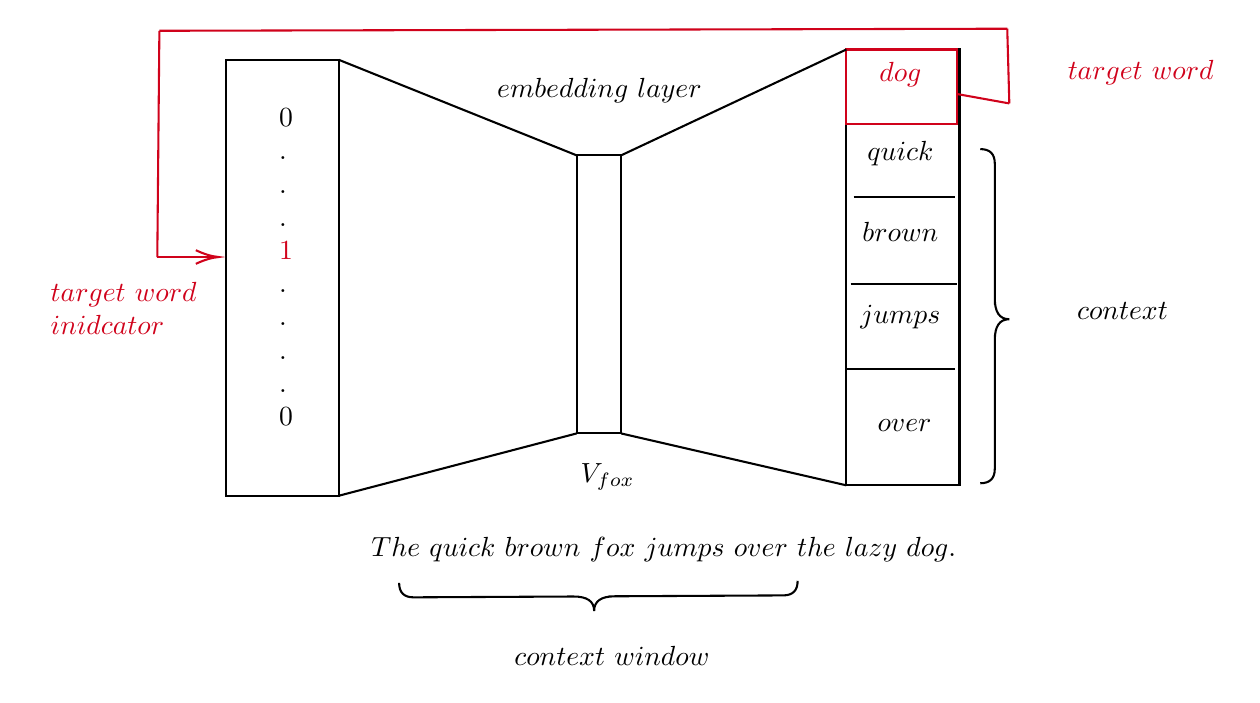
\begin{tikzpicture}[x=0.75pt,y=0.75pt,yscale=-1,xscale=1]
%uncomment if require: \path (0,347); %set diagram left start at 0, and has height of 347

%Shape: Rectangle [id:dp34856826620420023] 
\draw   (288,66) -- (309.5,66) -- (309.5,200) -- (288,200) -- cycle ;
%Shape: Rectangle [id:dp20385411601802828] 
\draw   (418,15) -- (472.5,15) -- (472.5,225) -- (418,225) -- cycle ;
%Shape: Rectangle [id:dp597929679831426] 
\draw  [color={rgb, 255:red, 208; green, 2; blue, 27 }  ,draw opacity=1 ] (418,15) -- (471.5,15) -- (471.5,51) -- (418,51) -- cycle ;
%Straight Lines [id:da329141353304766] 
\draw    (421.5,86) -- (470.5,86) ;


%Shape: Brace [id:dp7412735560954036] 
\draw   (202.5,272) .. controls (202.53,276.67) and (204.87,278.99) .. (209.54,278.96) -- (286.44,278.56) .. controls (293.11,278.53) and (296.45,280.84) .. (296.48,285.51) .. controls (296.45,280.84) and (299.77,278.49) .. (306.44,278.46)(303.44,278.47) -- (387.54,278.03) .. controls (392.21,278) and (394.53,275.66) .. (394.5,270.99) ;
%Straight Lines [id:da1987933863065281] 
\draw    (420,128) -- (471.5,128) ;


%Straight Lines [id:da8961013192322056] 
\draw    (418.5,169) -- (470.5,169) ;


%Shape: Brace [id:dp8413236825652046] 
\draw   (482.5,224) .. controls (487.17,224) and (489.5,221.67) .. (489.5,217) -- (489.5,154.97) .. controls (489.5,148.3) and (491.83,144.97) .. (496.5,144.97) .. controls (491.83,144.97) and (489.5,141.64) .. (489.5,134.97)(489.5,137.97) -- (489.5,70) .. controls (489.5,65.33) and (487.17,63) .. (482.5,63) ;
%Shape: Rectangle [id:dp5223635802427213] 
\draw   (119,20) -- (173.5,20) -- (173.5,230) -- (119,230) -- cycle ;
%Straight Lines [id:da26424324688833556] 
\draw [color={rgb, 255:red, 208; green, 2; blue, 27 }  ,draw opacity=1 ]   (86,115) -- (113.5,115) ;
\draw [shift={(115.5,115)}, rotate = 180] [color={rgb, 255:red, 208; green, 2; blue, 27 }  ,draw opacity=1 ][line width=0.75]    (10.93,-3.29) .. controls (6.95,-1.4) and (3.31,-0.3) .. (0,0) .. controls (3.31,0.3) and (6.95,1.4) .. (10.93,3.29)   ;

%Straight Lines [id:da3427921645180725] 
\draw [color={rgb, 255:red, 208; green, 2; blue, 27 }  ,draw opacity=1 ]   (87,6) -- (86,115) ;


%Straight Lines [id:da5378893688694539] 
\draw [color={rgb, 255:red, 208; green, 2; blue, 27 }  ,draw opacity=1 ]   (87,6) -- (495.5,5) ;


%Straight Lines [id:da1316572119067576] 
\draw [color={rgb, 255:red, 208; green, 2; blue, 27 }  ,draw opacity=1 ]   (495.5,5) -- (496.5,41) ;


%Straight Lines [id:da7079049036395544] 
\draw [color={rgb, 255:red, 208; green, 2; blue, 27 }  ,draw opacity=1 ]   (471.5,36.5) -- (496.5,41) ;


%Straight Lines [id:da6232994776605181] 
\draw    (173.5,20) -- (288,66) ;


%Straight Lines [id:da1671416061216935] 
\draw    (173.5,230) -- (288,200) ;


%Straight Lines [id:da8246799797542117] 
\draw    (309.5,66) -- (418,15) ;


%Straight Lines [id:da7881561473504775] 
\draw    (309.5,200) -- (418,225) ;



% Text Node
\draw (330,256) node   {$The\ quick\ brown\ fox\ jumps\ over\ the\ lazy\ dog.$};
% Text Node
\draw (303,221) node   {$V_{fox}$};
% Text Node
\draw (299,35) node   {$embedding\ layer$};
% Text Node
\draw (562,26) node [color={rgb, 255:red, 208; green, 2; blue, 27 }  ,opacity=1 ]  {$target\ word\ $};
% Text Node
\draw (444,27) node [color={rgb, 255:red, 208; green, 2; blue, 27 }  ,opacity=1 ]  {$dog$};
% Text Node
\draw (444,65) node   {$quick$};
% Text Node
\draw (444,103) node   {$brown$};
% Text Node
\draw (444,144) node   {$jumps$};
% Text Node
\draw (446,196) node   {$over$};
% Text Node
\draw (551,141) node   {$context$};
% Text Node
\draw (305,307) node   {$context\ window$};
% Text Node
\draw (148,121) node   {$ \begin{array}{l}
0\\
.\\
.\\
.\\
\textcolor[rgb]{0.82,0.01,0.11}{1}\\
.\\
.\\
.\\
.\\
0
\end{array}$};
% Text Node
\draw (72,141) node [color={rgb, 255:red, 208; green, 2; blue, 27 }  ,opacity=1 ]  {$ \begin{array}{l}
target\ word\ \\
inidcator
\end{array}$};


\end{tikzpicture}

}
\caption{Skip-gram architecure for the example sentence \emph{``The quick brown fox jumps over the lazy dog"}. }
\label{fig:skip_w2v}
\end{figure}
\noindent
\textbf{The skip-gram} objective is to train word vector representations that are good at predicting the nearby words. A visual representation of the skip-gram model can be seen in Figure~\ref{fig:skip_w2v} for the sentence \emph{``The quick brown fox jumps over the lazy dog"}, where the meaning of the word \emph{``fox"} is defined by the words in the window around it. The input is the one-hot vector for the the target word and the output is the context words.\\
More formally, given a corpus of words $f$ and their contexts $c$, to set the parameters $w$ of $p(c|a; w)$ so as to maximize the corpus probability, where $Q$ is the set of all focal (center) and context pairs extracted from the text. Equation~\ref{eq:w2v_p} shows the probability formulation.
\begin{equation}
\label{eq:w2v_p}
w^*=\underset { w  }{ { argmax } } \prod _{ (w,c)\in \quad Q }^{  }{ p(c|f; } w )
\end{equation}
The literature on neural-network language models, models this probablity using softmax shown in Equation~\ref{eq:w2v_softmax}, where $w_c$ and $ w_a\in R^d$ are vector representations for $c$ and $a$ respectively, and
$C$ is the set of all available contexts. The goal is to find the parameters $w$ such that Equation~\ref{eq:w2v_p} is maximized~\brackettext{\cite{DBLP:journals/corr/GoldbergL14}}. 
\begin{equation}
\label{eq:w2v_softmax}
p(c|a;w)=\frac { { e }^{ w_{ c }.w_{ a } } }{ \sum _{ \acute { a } \in C }^{  }{ { e }^{ w_{ c }.w_{ \acute { a }  } } }  } 
\end{equation}
Maximizing the log-likelihood of Equation~\ref{eq:w2v_softmax} on the training set is very expensive. Because we need to compute and normalize each probability using the score for all other words  $\acute { f }$ in the context of $c$. Therefore, the authors reformulate the problem using \emph{Negative Sampling}~\brackettext{\cite{DBLP:journals/jmlr/GutmannH12}}~\footnote{ In order to deal with the expensive computation of the softmax, the multinomial classification problem (predicting the next word) is converted into a binary classification problem. To estimate a true probability distribution of the output word, a binary logistic regression is used, where the classifier learns to distinguish between  a true pair (true context words) and randomly selected words from the vocabulary (corrupted pairs). The classifier simply predicts whether a pair of words is a true or a random sample. } to Equation~\ref{eq:w2v_negative}. $ \sigma$ shows the sigmoid function and $\acute{Q}$ is the set of random $(f, c)$ pairs, assuming they are all incorrect. By maximizing this objective, the model assigns high probabilities to the real word pairs, and low probabilities to noise word pairs and it is more computationally appealing than the softmax function.

\begin{equation}
\label{eq:w2v_negative}
\underset { w }{ { argmax } } \quad \sum _{ (c,f)\in Q }^{  }{ \log { \quad \sigma ( } w_{ c }.w_{ a }) } +\sum _{ (c,f)\in \acute { Q }  }^{  }{ \log { \quad \sigma ( } -w_{ c }.w_{ f })\quad  } 
\end{equation}
If the model is trained on enough data, word2vec groups the vectors of similar words together in vector space, finds word’s associations and detects similarities mathematically with cosine similarity. 
\subsection{GloVe: Global Vector Embeddings}
\label{subsec:GloVe}
The \emph{Global Vector Model} (GloVe) suggests that the ratio of co-occurrence probabilities can encode meaning components. An example can be seen in Table~\ref{table:tab_1}, in terms of studying a thermodynamic phase. A meaning component that sets the word  \emph{``ice''} apart from \emph{``steam''} can be represented as  a ratio of their occurrence probability with all other words \big($\frac { P(ice|k) }{ P(steam|k) } $, where $k$ can be any word in the vocabulary\big). This ratio is proved to better distinguish relevant words in comparison from irrelevant ones by giving the irrelevant ones a probability close to one. Also compared to the raw probabilities, it is better able to discriminate
between the relevant words by giving a high probability to a word like "solid" and low probability to \emph{``gas''}, making the word \emph{``ice'} stand out as a solid object. A word such as "\emph{``water''} or \emph{``fashion''} will, therefore, have a probability close to one as it is either a shared property or not related to the concept.\\
\begin{table}[]
\centering

\begin{tabular}{@{}l|l|l|l|l@{}}
\toprule
Probability and Ratio &  $k=solid$& $k=gas$ & $k=water$ &$k= fashion$  \\ \midrule $P(k|ice)$& {\color[HTML]{CB0000}large} &  {\color[HTML]{329A9D}small} & {\color[HTML]{CB0000}large} & {\color[HTML]{329A9D}small} \\\midrule
  $P(k|steam)$&{\color[HTML]{329A9D}small}  & {\color[HTML]{CB0000}large} &  {\color[HTML]{CB0000}large}&{\color[HTML]{329A9D}small}  \\\midrule
 $\frac { P(ice|k) }{ P(steam|k) } $& {\color[HTML]{CB0000}large} &  {\color[HTML]{329A9D}small}&  1 &    1  \\\midrule
\end{tabular}%
\caption{Co-occurrence probabilities for target words \emph{``ice'}and \emph{``steam'} with selected context words. Example taken from~\brackettext{\cite{DBLP:conf/emnlp/PenningtonSM14}}.}
\label{table:tab_1}
\end{table}
\noindent
To capture these ratios, the authors of GloVe propose a log-bilinear model, where, if the dot product of two vectors corresponds to the log of their co-occurrence probability, their difference will show the meaning component, as seen in Equation~\ref{eq:log_prob}.

\begin{equation}
\begin{split}
\\ w_{ i }.w_{ j }=\log { P(i|j)\quad  } \\ w_{ x }(w_{ i }-w_{ j })=\log { \frac { P(x|j) }{ P(x|j) } \quad  } 
\end{split}
\label{eq:log_prob}
\end{equation}
Based on the log-bilinearity assumption, the cost function is defined as follows:\\
Let the matrix of word-word co-occurrence counts be denoted by $X\in { R }^{ V\times V }$, where $V$ is the size of the vocabulary. Entries $X_{ij}$ tabulate the number of times word $j$ occurs in the context of word $i$. $w_{ i }\in { R }^{ 1\times M }$ and $\tilde{w_{ j }}\in { R }^{ 1\times M }$ are the focal (center word) and context embeddings, respectively, where $M$ is the embedding size. The model tries to learn embeddings that minimize the squared difference between the dot product of the center word embedding and context embedding to the logarithm of its co-occurrence.  \\
Considering $ \tilde{b_{ j }}$ and $b_{ i }$  as the biases for the focal and context embeddings. The cost function is defined in Equation~\ref{eq:glove_cost}.  Since the log of co-occurrences does not directly result into a probability, in order for the meaning component to have a probabilistic interpretation, a normalization factor is needed. Bias $b_{ i }$ allows the model to learn this constant during training and $ \tilde{b_{ j }}$ is added to preserve symmetry. 
\begin{equation}
J=\sum _{ i,j=1 }^{ V }{ f({ X }_{ ij } } )(w_{ i }^{ T }\tilde{  w_{ j } } +b_{ i }+\tilde{  b_{ j } } -log{ X }_{ ij })^2
\label{eq:glove_cost}
\end{equation}
Optimizing for the co-occurrence counts alone might cause the model to overemphasize the most common words. Therefore, a weighing function $f$ is introduced that imposes an upper bound on the maximum number of occurrences of a word. Conceptually,  $f$ scales the counts in order to avoid the influence of common words and boost the rare words. The choice of $f$ is not fixed but one class of functions that were used by the authors can be parametrized with $\alpha$ as the exponential weight and $x_{max}$ as the maximum number of allowed co-occurrences. $\alpha$ and $x_{max}$ are hyper-parameters that requires tuning, but the values suggested by the authors are for $\alpha$ is $\frac{3}{4}$ and for $x_{max}$ is $100$. 
\begin{equation}
f=\left\{
  \begin{array}{@{}ll@{}}
    (\frac { x }{ { x }_{ max } } )^{ \alpha  }& \text{if}\ x<x_{max} \\
    1 & \text{otherwise}
  \end{array}\right.
\label{eq:weighingfunction}
\end{equation}
\noindent
The model learns two embeddings for each word: one as a focal or center word and the other as a context word. As the co-occurrence matrix is symmetric both of which can be considered as learning the same representation. Ultimately, the two embeddings can be added to obtain the final embedding.

\subsection{Weights of the LOAD Resemble Co-occurrence Probabilities}
The cost function of the GloVe model is based on the assumption that the ratio of co-occurrence probabilities result in meaningful components, which can be investigated to find the relation between two words. Although edges of the LOAD network do not directly count co-occurrences in a given window, they relate closely to it. \\
The sentence distance is a more efficient way to define a distance metric between two entities rather than a window-based approach. As two entities appearing in the same document tend to have some connection, this relationship is disregarded, if we only look at a small window of words. Additionally, weights decay based on how far an entity is from another gives us more information about the structure of the text. Based on these considerations, we argue that LOAD edge weights produce a better overall corpus statistics in case of named entities with respect to a simple co-occurrence matrix and that it can generate the same meaningful components like probability ratios. \\
We demonstrate this with a simple example in Table~\ref{table:tab_2} that shows
how certain aspects of meaning can be extracted from edge weights of LOAD.  Suppose we are interested in the concept of US presidents, for which we take two actors \emph{``Donald Trump''} and \emph{``Barack Obama''}. The relationship between these entities can be examined by studying the ratio of their edge weights with various probe words. Similar to the GloVe model, where the ratio of co-occurrence probability distinguished the relevant words from irrelevant words, here the ratio of the edge weights works in the same way. In this case, looking at the raw edge weights does not give us much comparable information, but the ratio denotes \emph{``Donald Trump''} as a Republican rather than a democratic politician. Since both of the entities share the presidential attribute the ratio is close to one. On the other hand, a random name like \emph{``BMW''} has a relatively small weight with both entities, but since the weak edges were cut off from the model we have the weight of zero. Considering the full graph without a cut off threshold, the ratio of two small numbers will also converge to one, implying that same as co-occurrence matrix, edge weights of LOAD contain these meaning components. Consequently, the bilinearity assumption of GloVe can be extended to the weighted adjacency matrix of LOAD. 
\begin{table}[]
\centering

\begin{tabular}{@{}l|l|l|l|l@{}}
\toprule
Probability and Ratio&  $k=Republican$& $k=Democratic$ & $k=president$ &$k= BMW$  \\ \midrule
 $P(k|Trump)$& {\color[HTML]{CB0000}10.51} &  {\color[HTML]{329A9D}5.30} & {\color[HTML]{CB0000}52} & {\color[HTML]{329A9D}0} \\\midrule
  $P(k|Obama)$&{\color[HTML]{329A9D}0.36}  & {\color[HTML]{CB0000}1.29} &  {\color[HTML]{CB0000}66}&{\color[HTML]{329A9D}0}  \\\midrule
 $\frac { P(Trump|k) }{ P(Obama|k) } $& {\color[HTML]{CB0000}29.2} &  {\color[HTML]{329A9D}4.10}&  0.78 &    0  \\\midrule
\end{tabular}%

\caption{LOAD weights for target words \emph{``Donald Trump''} and \emph{``Barack Obama''} with selected context words. }
\label{table:tab_2}
\end{table}
\label{sec:components_load}

\section{Graph-based Embeddings}
\label{sec:graph}
Graph embeddings convert a graph into a low dimensional space in which the graph information is preserved. Therefore, it is an effective and efficient way to compute features from a graph for machine learning algorithms. Based on the embedding output, graph embeddings are categorized into four types: \emph{node embedding}, \emph{edge embedding}, \emph{hybrid embedding} (combination of different types of graph components, e.g, node $+$ edge) , and  \emph{whole-graph embedding} (a graph is represented as one vector)~\brackettext{\cite{DBLP:journals/tkde/CaiZC18}}. Different node embedding models vary in their definition of similarity between nodes and the graph property they preserve. Two of the most important properties are \emph{first-order proximity} and \emph{second-order proximity}. First-order proximity captures the direct neighbourhood relationship (edges) in a graph. Second-order proximity captures the $2$-end step relations (number of common neighbors shared). The second-oder proximity can also be extended to take higher orders into account as well. ~\brackettext{\cite{DBLP:journals/jmlr/GutmannH12}}.\\
Since the nodes of the co-occurrence graph correspond to words in the vocabulary, in this study we only look at node embedding techniques. Embedding the edges or whole graph does not provide any information about the words of the corpus. In the following we give a brief introduction into popular node embedding methods. 
\subsection{DeepWalk, a Random Walk-based Embedding}
\label{subsec:DeepWalk}
\begin{figure}
\centering 
\resizebox{0.8\textwidth}{0.35\textwidth}{      
\input{images/DeepWalk.tex}
}
\caption{The workflow of DeepWalk. It first generates random walk sequences
from a graph, and then applies the skip-gram model to learn the embeddings. Figure adapted from~\brackettext{\cite{SCHOL:journal/IEEE/zahng} }}
\label{fig:deepwalk}
\end{figure}

The \emph{DeepWalk}~\brackettext{\cite{DBLP:conf/kdd/PerozziAS14}} model  learns latent representations of nodes of a network, using  local information obtained from fixed length
random walks. The model treats the nodes visited in the random walk as words and walk itself as  a sentence from the corpus. Then skip-gram is applied on the generated corpus to maximize the probability of visiting the neighbourhood of the node conditioned on its embedding. A visualization of workflow of DeepWalk is shown in Figure~\ref{deepwalk}.  In other words, the model tries to learn the embedding $w\in R^{ d} $, where $d$ is a small number of latent dimensions in comparison to the number of nodes. The model maximizes the probability of observing the last $k$
nodes and the next $k$ nodes in the random walk entered at node
$t_{i}$, by minimizing negative log the probablity as shown in the Equation~\ref{eq:dw}, to learn the node embedding $w$~\brackettext{\cite{DBLP:journals/kbs/GoyalF18}}.: 
\begin{equation}
J=-\log { P( } t_{ { i−k } },...,t_{ i−1 },t_{ i+1 },...,t_{ i+k }|w )
\label{eq:dw}
\end{equation}
Based on this approach, nodes that share similar neighbours in random walk sequences should be represented closely in the embedding space. Since the random walk in DeepWalk correspond to the \emph{Depth-first Sampling (DFS)}, it can preserve the second-order proximity. As a result, DeepWalk is good at keeping community structures. 
\subsection{Node2vec}
\label{subsec:node2vec}
\emph{Node2Vec}~\brackettext{\cite{DBLP:conf/kdd/GroverL16}} extends the random walk procedure of DeepWalk by defining a more flexible notion of a node’s neighborhood. There are mainly two node sampling strategies in random walk : \emph{Breadth-first Sampling (BFS)} and \emph{Depth-first Sampling (DFS)}, where the BFS focuses on the immediate neighbors of the node and DFS consists of sampled nodes sequentially sampled at increasing distances from the
source node ~\brackettext{\cite{DBLP:conf/kdd/GroverL16}}. Therefore, BFS represents the first-order proximity and DFS the second and higher-order proximity. A demonstration of different sampling methods is provided in Figure~\ref{fig:dfs_bfs}. Node2vec provides a trade-off between BFS and DFS. Node2vec uses two hyperparameters to regulate the balance between the two methods. By choosing a right balance between the two sampling methods, we preserve community structure as well as structural equivalence
between nodes~\brackettext{\cite{DBLP:journals/kbs/GoyalF18}}. However, the node2vec method tends to be quite inefficient for large graphs and incurs significant space and time overhead. It runs out of memory even for mid-sized graphs. Although there exist complex graph strutures to speed up the proccess, the original model on large graphs is very slow~\brackettext{\cite{DBLP:journals/corr/abs-1805-00280}}. 
\begin{figure}
\centering 
\resizebox{0.45\textwidth}{0.25\textwidth}{      
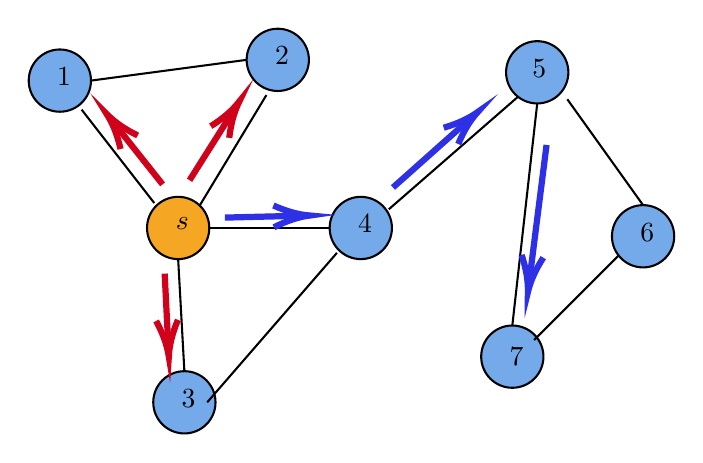
\begin{tikzpicture}[x=0.75pt,y=0.75pt,yscale=-1,xscale=1]
%uncomment if require: \path (0,407); %set diagram left start at 0, and has height of 407

%Shape: Circle [id:dp332493301566809] 
\draw  [fill={rgb, 255:red, 74; green, 144; blue, 226 }  ,fill opacity=0.77 ] (56,81) .. controls (56,72.72) and (62.72,66) .. (71,66) .. controls (79.28,66) and (86,72.72) .. (86,81) .. controls (86,89.28) and (79.28,96) .. (71,96) .. controls (62.72,96) and (56,89.28) .. (56,81) -- cycle ;
%Shape: Circle [id:dp4879070023914207] 
\draw  [fill={rgb, 255:red, 245; green, 166; blue, 35 }  ,fill opacity=1 ] (113,152) .. controls (113,143.72) and (119.72,137) .. (128,137) .. controls (136.28,137) and (143,143.72) .. (143,152) .. controls (143,160.28) and (136.28,167) .. (128,167) .. controls (119.72,167) and (113,160.28) .. (113,152) -- cycle ;
%Shape: Circle [id:dp5810034132491635] 
\draw  [fill={rgb, 255:red, 74; green, 144; blue, 226 }  ,fill opacity=0.77 ] (161,71) .. controls (161,62.72) and (167.72,56) .. (176,56) .. controls (184.28,56) and (191,62.72) .. (191,71) .. controls (191,79.28) and (184.28,86) .. (176,86) .. controls (167.72,86) and (161,79.28) .. (161,71) -- cycle ;
%Shape: Circle [id:dp678091001536465] 
\draw  [fill={rgb, 255:red, 74; green, 144; blue, 226 }  ,fill opacity=0.77 ] (116,236) .. controls (116,227.72) and (122.72,221) .. (131,221) .. controls (139.28,221) and (146,227.72) .. (146,236) .. controls (146,244.28) and (139.28,251) .. (131,251) .. controls (122.72,251) and (116,244.28) .. (116,236) -- cycle ;
%Shape: Circle [id:dp19856877490785307] 
\draw  [fill={rgb, 255:red, 74; green, 144; blue, 226 }  ,fill opacity=0.77 ] (201,152) .. controls (201,143.72) and (207.72,137) .. (216,137) .. controls (224.28,137) and (231,143.72) .. (231,152) .. controls (231,160.28) and (224.28,167) .. (216,167) .. controls (207.72,167) and (201,160.28) .. (201,152) -- cycle ;
%Shape: Circle [id:dp06052439820005162] 
\draw  [fill={rgb, 255:red, 74; green, 144; blue, 226 }  ,fill opacity=0.77 ] (286,77) .. controls (286,68.72) and (292.72,62) .. (301,62) .. controls (309.28,62) and (316,68.72) .. (316,77) .. controls (316,85.28) and (309.28,92) .. (301,92) .. controls (292.72,92) and (286,85.28) .. (286,77) -- cycle ;
%Shape: Circle [id:dp7842135850860721] 
\draw  [fill={rgb, 255:red, 74; green, 144; blue, 226 }  ,fill opacity=0.77 ] (274,214) .. controls (274,205.72) and (280.72,199) .. (289,199) .. controls (297.28,199) and (304,205.72) .. (304,214) .. controls (304,222.28) and (297.28,229) .. (289,229) .. controls (280.72,229) and (274,222.28) .. (274,214) -- cycle ;
%Shape: Circle [id:dp69600261549569] 
\draw  [fill={rgb, 255:red, 74; green, 144; blue, 226 }  ,fill opacity=0.77 ] (337,156) .. controls (337,147.72) and (343.72,141) .. (352,141) .. controls (360.28,141) and (367,147.72) .. (367,156) .. controls (367,164.28) and (360.28,171) .. (352,171) .. controls (343.72,171) and (337,164.28) .. (337,156) -- cycle ;
%Straight Lines [id:da49057224619926565] 
\draw    (81.5,95) -- (116.5,140) ;


%Straight Lines [id:da40111900668895095] 
\draw    (128,167) -- (131,221) ;


%Straight Lines [id:da3149529915409619] 
\draw    (170.5,88) -- (138.5,141) ;


%Straight Lines [id:da40356254390150004] 
\draw    (143,152) -- (201,152) ;


%Straight Lines [id:da11721701648427074] 
\draw    (142,236) -- (204.5,164) ;


%Straight Lines [id:da7531222279660781] 
\draw    (86,81) -- (161,71) ;


%Straight Lines [id:da6126183155613649] 
\draw    (291.5,89) -- (229.5,143) ;


%Straight Lines [id:da4426831658921855] 
\draw    (315.5,90) -- (352,141) ;


%Straight Lines [id:da44944128673840367] 
\draw    (301,92) -- (289,199) ;


%Straight Lines [id:da49417599304234616] 
\draw    (340.5,165) -- (299.5,206) ;


%Straight Lines [id:da9093872174761735] 
\draw [color={rgb, 255:red, 208; green, 2; blue, 27 }  ,draw opacity=1 ][line width=2.25]    (120.5,131) -- (95.99,100.13) ;
\draw [shift={(93.5,97)}, rotate = 411.55] [color={rgb, 255:red, 208; green, 2; blue, 27 }  ,draw opacity=1 ][line width=2.25]    (17.49,-5.26) .. controls (11.12,-2.23) and (5.29,-0.48) .. (0,0) .. controls (5.29,0.48) and (11.12,2.23) .. (17.49,5.26)   ;

%Straight Lines [id:da13977987756203492] 
\draw [color={rgb, 255:red, 208; green, 2; blue, 27 }  ,draw opacity=1 ][line width=2.25]    (133.5,129) -- (155.36,94.38) ;
\draw [shift={(157.5,91)}, rotate = 482.28] [color={rgb, 255:red, 208; green, 2; blue, 27 }  ,draw opacity=1 ][line width=2.25]    (17.49,-5.26) .. controls (11.12,-2.23) and (5.29,-0.48) .. (0,0) .. controls (5.29,0.48) and (11.12,2.23) .. (17.49,5.26)   ;

%Straight Lines [id:da447165384934876] 
\draw [color={rgb, 255:red, 208; green, 2; blue, 27 }  ,draw opacity=1 ][line width=2.25]    (121.5,174) -- (123.3,210) ;
\draw [shift={(123.5,214)}, rotate = 267.14] [color={rgb, 255:red, 208; green, 2; blue, 27 }  ,draw opacity=1 ][line width=2.25]    (17.49,-5.26) .. controls (11.12,-2.23) and (5.29,-0.48) .. (0,0) .. controls (5.29,0.48) and (11.12,2.23) .. (17.49,5.26)   ;

%Straight Lines [id:da7666273172002611] 
\draw [color={rgb, 255:red, 46; green, 48; blue, 230 }  ,draw opacity=1 ][line width=2.25]    (150.5,147) -- (187.5,146.1) ;
\draw [shift={(191.5,146)}, rotate = 538.6] [color={rgb, 255:red, 46; green, 48; blue, 230 }  ,draw opacity=1 ][line width=2.25]    (17.49,-5.26) .. controls (11.12,-2.23) and (5.29,-0.48) .. (0,0) .. controls (5.29,0.48) and (11.12,2.23) .. (17.49,5.26)   ;

%Straight Lines [id:da7337308124937729] 
\draw [color={rgb, 255:red, 46; green, 48; blue, 230 }  ,draw opacity=1 ][line width=2.25]    (231.5,132.5) -- (269.51,98.66) ;
\draw [shift={(272.5,96)}, rotate = 498.32] [color={rgb, 255:red, 46; green, 48; blue, 230 }  ,draw opacity=1 ][line width=2.25]    (17.49,-5.26) .. controls (11.12,-2.23) and (5.29,-0.48) .. (0,0) .. controls (5.29,0.48) and (11.12,2.23) .. (17.49,5.26)   ;

%Straight Lines [id:da34116815343810125] 
\draw [color={rgb, 255:red, 46; green, 48; blue, 230 }  ,draw opacity=1 ][line width=2.25]    (305.5,112) -- (297,179.03) ;
\draw [shift={(296.5,183)}, rotate = 277.22] [color={rgb, 255:red, 46; green, 48; blue, 230 }  ,draw opacity=1 ][line width=2.25]    (17.49,-5.26) .. controls (11.12,-2.23) and (5.29,-0.48) .. (0,0) .. controls (5.29,0.48) and (11.12,2.23) .. (17.49,5.26)   ;


% Text Node
\draw (73,79) node   {$1$};
% Text Node
\draw (130,150) node   {$s$};
% Text Node
\draw (178,69) node   {$2$};
% Text Node
\draw (133,234) node   {$3$};
% Text Node
\draw (218,150) node   {$4$};
% Text Node
\draw (302,75) node   {$5$};
% Text Node
\draw (291,214) node   {$7$};
% Text Node
\draw (354,154) node   {$6$};


\end{tikzpicture}

}
\caption{DFS and BFS sampling for a random walk with lenght $3$ from the start node \emph{``s"}. The figure is adapted from ~\brackettext{\cite{DBLP:conf/kdd/GroverL16} }}
\label{fig:dfs_bfs}
\end{figure}

\subsection{LINE: Large-scale Information Network Embedding}
\label{subsec:LINE}
The \emph{LINE} model~\brackettext{\cite{DBLP:conf/www/TangQWZYM15}}, does not use random walks, instead optimizes two objective functions, one each for
first- and second-order proximities, and minimizes the combination
of the two to achieve two embeddings. The first objective function aims to keep the adjacency matrix and dot product of embeddings close. The LINE model defines
two joint probability distributions for each pair of nodes, one
using adjancency matrix and the other using the embedding and minimizes the \emph{Kullback-Leibler (KL) divergence}~\footnote{A measure of how one probability distribution is different from another.} of the distributions. The first objective results into the first half of the embedding. The authors define probability distributions and
objective function for the second half based on the the second-order proximity~\brackettext{\cite{DBLP:journals/kbs/GoyalF18}}. Nevertheless, the model fails to learn meaningful representation of graphs with unbalanced edge weights. The objective function for the second-order proximity is ill-defined for when the weight
of edges have a high variance~\brackettext{\cite{DBLP:conf/www/TangQWZYM15}}. 
\subsection{VERSE: Versatile Graph Embeddings from Similarity Measures}
\label{subsec:VERSE}
The \emph{VERSE}~\brackettext{\cite{DBLP:conf/www/TsitsulinMKM18}} model learns embeddings by training a single-layer neural network, which can be instantiated with
diverse similarity measures.  Given a graph $G=(T,E)$, where $T$ is the set of nodes and $E$ the set of all edges, the aim is to learn  the node embedding $w \in R^{d}$ , where $d$ is small number of latent dimensions, by optimizing the objective function in Equation~\ref{eq:VERSE}. In optimization objective, the KL-divergence from the given similarity distribution $sim_G$ to that of $sim_E$ in the embedded space is minimized, for any node $t$. 
\begin{equation}
\sum _{ t\in T }^{  }{ KL(sim_{ G }(t,.),sim_{ E } } (t,.))
\label{eq:VERSE}
\end{equation}
The similarity of two nodes in the embedding space is related to their dot product in the embedding space. Therefore, the similarity distribution ( $sim_E$) between two nodes $t$ and $v$ in the embedded space is their dot product ($w_t . w_v$), normalized with softmax, as shown in Equation~\ref{eq:VERSE_simE}. We should minimize the KL-divergence between the $sim_{ E }$ and an arbitrary similarity measure for the nodes to produce node embeddings. 
\begin{equation}
sim_{ E }(t,.)=\frac{ w_{ t }.W^{ T } }{ \sum _{ i=1 }^{ n }{ exp(w_{ t }.w_{ i }) }  }\label{eq:VERSE_simE}
\end{equation}
Although VERSE is designed to accept any similarity measure, three measures are contained in the original implementation: \emph{Personalized PageRank (PPR)},  \emph{Adjacency Similarity}, and  \emph{SimRank}. PPR is based on the stationary distribution of a random walk with restart. Thus, this measure is closely related to DeepWalk and node2vec. SimRank is a measure of structural relatedness. If two nodes are connected to similar nodes they are themselves considered similar. Adjacency Similarity is based on the normalized adjacency matrix. More formally, given the out degree $Out(t_{i})$ of node $t_{i}$, $sim_{ G }$ for the Adjacency Similarity is shown in Equation~\ref{eq:VERSE_simG}~\brackettext{\cite{DBLP:conf/www/TsitsulinMKM18}}. 
\begin{equation}
sim^{ ADJ }_{ G }(t_{ i },t_{ j })=\left\{ \begin{matrix} \frac { 1 }{ Out(t_{ i }) } \quad if\quad (t_{ i },t_{ j })\in E\quad  \\ 0\quad \qquad \qquad otherwise \end{matrix} \right.\label{eq:VERSE_simG}
\end{equation}
Since the optimization objective is expensive, the \emph{VERSE} samples positive and negative samples with \emph{Noise Contrastive Estimation (NCE)}~\footnote{This is same as Negative Sampling used in word2vec. The difference is that in word2vec words for the negative samples are drawn from a specially designed distribution, which favors less frequent words. }~\brackettext{\cite{DBLP:journals/jmlr/GutmannH12}} to converge to a solution. \\
\\
\ornament
In the next section, we use these background information for the  word embedding and graph embedding techniques to define our entity embedding and faceted embedding models. 
